\documentclass[../../main.tex]{subfiles}
% 
\begin{document}
\chapter{Častice a ich vzájomné interakcie}
\section{Zadanie}
Částice a jejich vzájemné interakce
Interakce mezi elementárními částicemi, Vlastnosti elementárních částic, Klasifikace elementárních částic, Hadrony, Leptony, Antičástice, Symetrie a zákony zachování, Standardní model, Zákony zachování energie a hybnosti, Souřadné soustavy v subjaderné fyzice, Transformace kinematických veličin mezi soustavami, Mandelstamovy proměnné, Kinematické proměnné – rapidita. pseudorapidita, Feynmanova proměnná, Bjorkenova proměnná

%OOOOOOOOOOOOOOOOOOOOOOOOOOOOOOOOOOOOOOOOOOOOO
%OOOOOOOOOOOOOOOOOOOOOOOOOOOOOOOOOOOOOOOOOOOOO
%OOOOOOOOOOOOOOOOOOOOOOOOOOOOOOOOOOOOOOOOOOOOO
\section{Štandardný model}
\subsection{História}
V roku 1960 navrhol Sheldon Glashow teoretickú možnosť ako skombinovať elektromagnetickú a slabú interakciu do jednotnej teórie. O sedem rokov neskôr doplnili Steven Weinberg a Abdus Salam navrhnutý teoretický model o Higgsov mechanizmus, ktorý priamo determinuje hmotnosti elementárnych častíc popísaných v rámci štandardného modelu. Špeciálne ide hlavne o hmotnosti W a Z bozónov a fermiónov. Higgsov mechanizmus takisto vysvetľuje, akým spôsobom "získavajú" hmotnosť kvarky a leptóny.\par
Po objave slabých neutrálnych prúdov v CERNe, spôsobených výmenou Z bozónov sa elektroslabá teória stala široko akceptovanou. Glashow, Salam a Weinberg, tvorcovia tejto teórie, následne dostali v roku 1979 Nobelovú cenu za fyziku. Neskôr, v r. 1981 boli experimentálne objavené bozóny W a Z. Experimentálne boli určené ich hmotnosti, pričom tieto boli v dobrej zhode s predpoveďami poskytnutými Štandardným modelom.\par
Teória silnej interakcie získala svoju modernú podobu v rokoch 1973 – 74, kedy experimenty potvrdili, že hadróny sú zložené zo zlomkovo nabitých kvarkov.
\subsection{Prehľad}
Štandardný model fyziky častíc je zjednotený súbor teoretických poznatkov zahrňujúci väčšinu známych elementárnych častíc. V rámci modelu je možné zjednoteným spôsobom (zjednotenou matematickou formuláciou) popísať tri zo štyroch fundamentálnych interakcií: silnú, slabú, a elektromagnetickú. Štandardný model predstavuje relativistickú kvantovú teóriu vyhovujúcu zároveň princípom špeciálnej teórie relativity i kvantovej mechaniky. Gravitačná interakcie a teda ani všeobecná teória relativity nie su v modeli zahrnuté. Fundamentálnymi objektmi vystupujúcimi v tejto teórii sú polia v časopriestore. Štandardný model bol vypracovávaný postupne. Jeho základy boli položené začiatkom 20. storočia. Súčasná formulácia bola dokončená v 70-tych rokoch po experimentálnom potvrdení existencie kvarkov. Táto teória je v dobrom súlade so súčasnými experimentálnymi údajmi. Zahrňuje však 18 voľných parametrov, ktorých hodnotu nepredpovedá. Hodnota týchto parametrov je určená výhradne na základe experimentálnych výsledkov. Nepopisuje taktiež gravitáciu, tmavú hmotu či tmavú energiu.\par 
Štandardný model je kalibračná teória silných (SU(3)) a elektroslabých (SU(2)xU(1)) interakcií s kalibračnou grupou nazývanou tiež Štandardný model symetrickej grupy SU(3)xSU(2)xU(1).\par
V nasledujucej casti si povieme o elementarnych casticiach a interakciach medzi nimi.

\section{Elementárne častice a ich klasifikácia} 
Pod pojmom elementárna častica alebo fundamentálna častica rozumieme časticu, ktorej subštruktúra je neznáma, a teda nie je známe, či je zložená z iných častíc. Tieto častice můžou byt rozdelené do dvoch skupin: elementarne fermiony a bosony.
\subsection{Elementárne fermióny} 
Do tejto skupiny patria kvarky a leptony, ktore tvoria hmotu okolo nas preto ich mozme nazvat aj časticami hmoty. Rozdelenie tychto castic je nasledovne, pozri tabulku (\ref{sf1:fig:Tabulka_fermionov}).
\begin{figure}[!h]
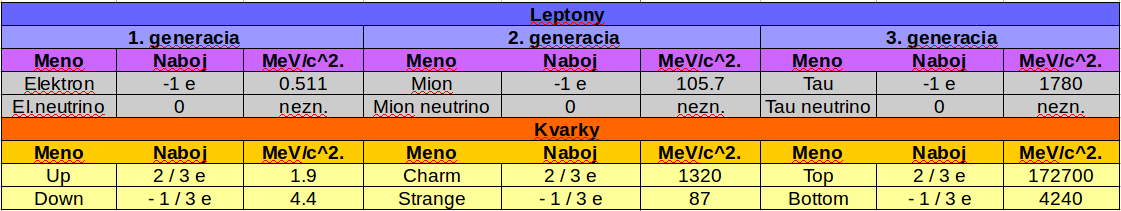
\includegraphics[width=1.0\textwidth]{Vlastnosti_tabulka.png}
\caption{Tabulka fermionov}
\label{sf1:fig:Tabulka_fermionov}
\end{figure}

Vsetky elementarne fermiony sú častice s poločíselným spinom (1/2), antisymetrickou vlnovou funkciou, splnaju Pauliho vylučovací princíp a ich správanie určuje Fermi-Diracovo rozdelenie, ktore je
\begin{equation}
f(\epsilon_i)=\frac{1}{e^{(\epsilon_i-\mu)/kT}+1},
\end{equation}
kde $k$ je Boltzmannova konštanta, $T$ je absolútna teplota, $\epsilon_i$ je energia jedno-časticoveho stavu $i$ a $\mu$ je celkový chemický potenciál (pre T=0 to je fermiho energia).\par
Nabité \textbf{leptóny} ($e^{-}$, $\mu^{-}$, $\tau^{-}$) interaguju elektromagnetickou a slabou interakciou zatial co neutrálne leptony (neutrina) interagujú iba slabou interakciou. Leptony neinteraguju silnou interakciou!\par
\textbf{Kvarky} interaguju silnou, slabou a elektromagnetickou interakciou. Každý kvark nesie jeden z troch farebných nábojov silnej interakcie (green, red, blue). Izolované kvarky neboli nikdy v prirode pozorované a vyskytuju sa len vo viazanych stavoch zvanych \textbf{hadrony}, ktore maju neutralny farebny naboj. Existujú stovky rôznych druhov hadrónov, niektoré sú takmer stabilné a niektoré (známe ako rezonancie) majú extrémne krátku životnosť. Stupeň stability závisí hlavne od hmotnosti hadrónu. Hadrony mozme rozdelit na baryony a mezony. 
\begin{itemize}
\item \textbf{Baryóny} su zložené částice, ktoré obsahuju 3 kvarky a majú polovičný spin, napr.(proton-uud, neutron-udd, $\Lambda$-uds). Baryón, ktorý obsahuje jeden alebo viac strange kvarkov, ale žiadny charm, bottom alebo top kvark, sa nazýva hyperón. Keďže silné interakcie si zachovávajú zvláštnosť (strangeness), hyperóny sa nemôžu rozpadnúť silnou interaktiou avsak zucastnuju sa silnej interakcie (to znamena, ze mozu vzniknut silnou interakciou). Rozpadaju sa niekolko-nasobnou slabou interakciou, ktora meni ich strangeness, povecsine na proton alebo neutron a ine castice (slaba interakcia podivnost nezachovava).
\item \textbf{Mezony} su zlozene z jedného kvarku a jedného antikvarku a vysledny mezon musi byt bezfarebny. Všetky mesóny sú nestabilné, pričom najdlhšia životnosť trvá len niekoľko stotín mikrosekúnd. Nabité mezóny sa rozpadaju na elektróny a neutrína (ako mozu sa rozpadnut aj na ine mezony ale tie sa potom tiez rozpadnu az to vacsinou skonci na leptonoch). Nenabité mezóny sa môžu rozpadnúť na fotóny. Obe tieto rozpady naznačujú, že farebny naboj už nie je vlastnosťou vedľajších produktov. Rozlisuju sa mezony skalarne (spiny kvarku a antikvarku su orientove opacne, takze vysledny spin mezonu je s = 0) a mezony vektorové (spin kvarku a antikvarku maju rovnaky smer, takže výsledný spin mezonu je s = 1). Mesony sa zaraduju medzi bosony, kedze maju celocisleny spin avsak nie medzi elementarne bosony. 
\end{itemize}
\subsection{Elementárne bozóny}
Su to častice, ktore zprostředkuvaju základne interakce; foton pro elektromagnetickou interakciu, bosony $W^{\pm}$, $Z^0$ pro slabu interakciu a gluony pro silnu interakciu.
Tieto castice maju celocisleny spin, symetricku vlnovu funkciu, nesplnaju Pauliho vvylucovani princip, a ich spravanie je riadene Bose-Einsteinovou statistikou, ktore ma tvar
\begin{equation}
f(\epsilon_i)=\frac{1}{e^{(\epsilon_i-\mu)/kT}-1}.
\end{equation}
Do tejto skupiny patri aj Higgsov boson, ktory ma spin = 0 a ktory je zodpovedný za hmotnost častíc.

\section{Fundamentálne interakcie}
Este nez pristupime k jednotlivemu popisu jednotlivych interakcii, uvedieme tabulku, v ktorej su zakladne charakteristiky fundamentalnych interakcii, obrazok \ref{sf1:fig:Tabulka_interakcie}
\begin{figure}[!h]
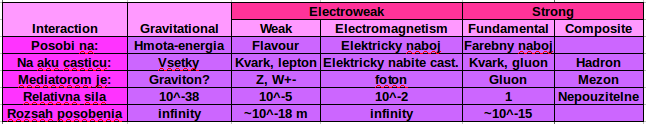
\includegraphics[width=1.0\textwidth]{Tabulka_interakcie.png}
\caption{Tabulka interakcii}
\label{sf1:fig:Tabulka_interakcie}
\end{figure}
\subsection{Elektromagnetická interakcia}
Prvou interakciou, ktorou sa budeme zaoberat, je elektromagnetická interakcia, ktorá posobi medzi časticami s nenulovým elektrickým nábojom. Mediatorom tajte interakcie je fotón, čo je vektorova častíce (spin = 1).

Opis tejto interakcie zacneme najprv z klasickeho hladiska. V klasickom elektromagnetisme se elektromagnetické pole riadí sadou rovnic známých jako Maxwellovy rovnice
\begin{equation}
\begin{gathered}
\nabla \cdot \vec{E} = \frac{\rho}{\epsilon_0}\\
\nabla \cdot \vec{B} = 0\\
\nabla \times \vec{E}=-\frac{\partial \vec{B}}{\partial t}\\
\nabla \times \vec{B}= \mu_0 \vec{j}+\mu_0\epsilon_0\frac{\partial \vec{E}}{\partial t}
\end{gathered}
\end{equation} 
Prvá rovnica opisuje, ako sú elektrické polia vyvolané nabojmi. Druhá rovnica hovorí, že neexistuje nič také ako magnetický monopol. Tretia rovnica opisuje indukciu elektrických polí zmenou magnetických polí a štvrtá rovnica opisuje generovanie magnetických polí elektrickými prúdmi a indukciu magnetických polí casovou zmenou elektrických polí.\par
Z druhej a tretej Maxwellovej rovnica sa navyse da ukazat, ze polia $\vec{E}$ a $\vec{B}$ mozu byt prepisane nasledovne 
\begin{equation}
\begin{gathered}
\vec{B} = \nabla \times \vec{A}\\
\vec{E} = -\nabla\varphi-\frac{\partial}{\partial t}\vec{A},
\end{gathered}
\end{equation}  
kde funkcia $\vec{A}$ sa nazyva vektorovy elektromagneticky potencial a funkcia $\varphi$ je skalarny elektromagneticky potencial. Skalarny a vektorovy potencial su urcene hustotami elektrickeho naboja a prudu prostrednıctvom rovnıc, ktore dostaneme zo zvysnych dvoch Maxwellovych rovnıc, ked do nich dosadime $\vec{B}$ a $\vec{E}$ vyjadrene cez dane potencialy. Co je vsak dolezitejsie je to, ze tieto potencialy nie su urcene jednoznacne. A tak mozme z potencialu $\vec{A}$ prejst na potencial 
\begin{equation}
\vec{A} \rightarrow \vec{A}+grad(\Lambda).
\end{equation}
Toto mozme urobit preto lebo rotacia gradientu akejkolvek vektorovej funkcie je vzdy nula, takze nase $\vec{B}$ sa vobec nezmeni. Nasledne aby sa nezmenil ani skalarny potencial tak aj ten musi prejst z $\varphi$ na
\begin{equation}
\varphi \rightarrow \varphi -\frac{\partial}{\partial t}\Lambda
\end{equation}
. Touto transformaciou poli sa nezmeni ani $\vec{B}$ ani $\vec{E}$. Uvedena transformacia elmag potencialov (oboch sucasne!) sa nazyva \textbf{kalibracna transformacia}.\par
Preco sme to ale vlastne cele robili a zaviedli sme taketo potencialy? Odpovedou napriklad je, ze kvantova mechanika castice v elmag. poli je opısana Schrodingerovou rovnicou, v ktorej vystupuju elmag potencialy a nie elmag polia. Nahradenie elmag potencialov elmag. poliami by tu bolo znacne komplikovane a neprirodzene. Navyse kvantova teoria samotneho elmag. pola, tzv. kvantova elektrodynamika, je
zalozena na tzv. kvantovanı klasickej teorie. K tomuto kvantovaniu je potrebne mat sformulovanu klasicku elektrodynamiku v lagrangeovskom alebo hamiltonovskom
formalizme. Pre oba tieto formalizmy su elmag. potencialy ovela vhodnejsie a prirodzenejsie ako elmag. polia.\par
Problémy klasického elektromagnetismu nastaly ked Einstein publikoval teoriu fotoelektrického javu, v ktorej predpoklada, že svetlo se nešírí ako vlnenie elektromagnetického pola, ale može existovat ve forme částic, diskrétních kvant, neskor nazývaných fotony. Einsteinova teoria fotoelektrického javu bola v sulade s predstavami, ktoré sa objavily v navrhnutom riešení Maxe Plancka v roku 1900. Vo svojej práci Planck predpokládal, že elektromagnetické vyzarovánie telies prebíehá cez diskrétne kvanta, což vedie ku konečnej celkovej energii. Tato predstava bola v priamom protiklade s klasickým pohladom na svetlo ako spojitu vlnu. Planckova a Einsteinova teorie následne viedly ku kvantovej mechanike, ktorá bola formulována v roce 1925. Na jej základe bola okolo roku 1940 dokončena nová kvantovo-mechanická teorie elektromagnetismu; kvantová elektrodynamika („QED“) a je jednou z nejpresnejších fyzikálních teorií.\par
\textbf{Kvantová elektrodynamika} je nauka o pohybe elektrických nábojov (nabitých telies) v obecne premenných elektromagnetických poliach. Klasická elektrodynamika studuje elektrodynamické interakce medzi makroskopickými telesami, kvantová elektrodynamika interakce medzi mikro-objektmy. QED popisuje interakciu ziarenia s hmotou (fotoelektrický jav, Comptonov rozptyl, brzdné ziarenie), elektromagnetické interakcie medzi nabitými elementárními částicami, reakce fotonov. Kvantová elektrodynamika vznikla ako teoria interakcie elektromagnetického pole a pole popisujíceho elektrony a pozitrony.\par
A podme teraz na samotny matematicky aparat QED. Tento bude trochu dlhsi ako tie dalsie dva a to len preto aby som demostroval silu tych kalibracnych transformacii. Zacneme velmi z lahka a to tym, ze si napiseme Diracov lagrangian pre diracovu volnu casticu (kde $c$=$h$=1).
\begin{equation}
\mathcal{L}_D=\bar{\psi}(i\gamma^{\mu}\partial_{\mu}-m)\psi
\end{equation}
Pomocou Euler–Lagrange rovnice pohybu pre pole, ktora ma tvar
\begin{equation}
\partial_{\mu}\bigg(\frac{\partial \mathcal{L}}{\partial(\partial_{\mu}\psi)}\bigg)-\frac{\partial\mathcal{L}}{\partial\psi}=0,
\end{equation}
sme schopny dostat Diracovu rovnicu v tvare
\begin{equation}
(i\gamma^{\mu}\partial_{\mu}-m)\psi=0.
\end{equation}
Toto je pohybova rovnice pre volny elektrony. V pripade pozitronu by sme dostali
\begin{equation}
\bar{\psi}(i\gamma^{\mu}\partial_{\mu}+m)=0.
\end{equation}
Z tychto dvoch rovnic (ked ich scitame a vynasobime $\bar{\psi}$, $\psi$) mozme odvodit rovnicu kontinuity (spojitosti) pre 4-vektor prudu
\begin{equation}
\partial_{\mu}j^{\mu}=0,
\end{equation}
kde $j=e\bar{\psi}\gamma^{\mu}\psi$.
Toto odvodenie bolo na klasickej hladine, v kvantovom pripade by to bolo uplne to iste len akurat by to musela byt normalne usporiadana nabojova hustota. Pre vacsie detaily ohladom tohto usporiadania pozri ($http://sophia.dtp.fmph.uniba.sk/~peterp/QED_A.pdf$).\par
Ako som uz spominal toto odvodenie bolo len pre volnu diracovu casticu, ktora s nicim neinteragovala. Teraz vsak budeme chciet aby s nasim nabitym polom $\psi$ interagovalo nejake dalsie pole. Ako ale pridat nejake dalsie pole tak aby sme nenarusili celu tuto konstrukciu? Mozme si vsimnut, ze fyzikálne veličiny ako hustota náboja ($\bar{\psi}\psi$) alebo prúd ($\bar{\psi}\gamma^{\mu}$) su invariantne ak pridame lokalnu fazu $\Lambda(x)$ do pola $\psi$.
\begin{equation}
\begin{gathered}
\psi(x)\rightarrow e^{iq\Lambda(x)}\psi(x)\\,
\bar{\psi(x)}\rightarrow e^{-iq\Lambda(x)}\bar{\psi(x)},
\end{gathered}
\end{equation}
tato transformacia sa nazyva lokalna U(1) kalibracna transformacia. Kebyze tuto transformaciu aplikujeme na clen $\bar{\psi}\partial_{\mu}\psi$ zistime, ze nie je invariantny pre tuto transformaciu pretoze derivacia ($\partial_{\mu}$) sa pod touto U(1) symetriou netransformuje invariantne. 
\begin{equation}
\bar{\psi}\partial_{\mu}\psi \rightarrow (\bar{\psi}e^{-iq\Lambda(x)})\partial_{\mu}(e^{iq\Lambda(x)}\psi)=\bar{\psi}(\partial_{\mu}+iq\Lambda(x))\psi\neq \bar{\psi}\partial_{\mu}\psi.
\end{equation}
Aby sme vyriesili nekovariantnost derivacie a spravili tak lagrangian kalibracne invariantny, musime zaviest kalibracne pole $A_{\mu}$ a to nasledovne
\begin{equation}
D_{\mu}=\partial_{\mu}-iqA_{\mu},
\end{equation}
kde ako uz vieme $A_{\mu}$ sa musi transformovat ako $A_{\mu}\rightarrow A_{\mu}+\partial_{\mu} \Lambda(x)$. $D_{\mu}$ sa nazyva kovariantna derivacia a je invariantna pod lokalnymi kalibracnymi trasnformaciami, co vlastne znamena
\begin{equation}
\bar{\psi}D_{\mu}\psi=\bar{\psi}(\partial_{\mu}-iqA_{\mu})\psi \rightarrow \bar{\psi}e^{-iq\Lambda(x)}(\partial_{\mu} - iq(A_{\mu}+\partial_{\mu}\Lambda(x)))e^{iq\Lambda(x)}\psi=\bar{\psi}D_{\mu}\psi.
\end{equation}
Ked teraz do lagrangianu pre volnu casticu vlozime tuto kovariantnu derivaciu namiesto normalnej parcialnej derivacie ($\partial_{\mu}\rightarrow D_{\mu}$) a vykoname na nom kalibracnu transformaciu vsetkych poli
\begin{equation}
\begin{gathered}
\psi \rightarrow e^{iq\Lambda(x)}\psi, \\
\bar{\psi} \rightarrow e^{-iq\Lambda(x)}\bar{\psi}, \\
A_{\mu}\rightarrow A_{\mu}+\partial_{\mu}\Lambda(x),
\end{gathered}
\end{equation}
tak dostaneme lagrangian, ktory mozme napisat tvare
\begin{equation}
\mathcal{L}=\bar{\psi}(i\gamma^{\mu}\partial_{\mu}-m)\psi+q\bar{\psi}\gamma^{\mu}\psi A_{\mu}.
\end{equation}
Ako mozme vidiet, tento lagrangian pozostava z povodneho Diracovho lagrangianu pre volnu casticu a noveho interakcneho clenu medzi polom castice a novym kalibracnehym polom. Symbol $q$ znaci elektricky naboj castice. Tento lagrangian uz obsahuje to co sme chceli akurat nie je kompletny a to z toho dovodu, ze mu chyba kineticky clen pre pole $A_{\mu}$. Tento clen sa da lahko dostat z Procovho lagrangianu, ten pouzijeme preto lebo pole $A_{\mu}$ musi reprezentovat vektorovu casticu
\begin{equation}
\mathcal{L}_{Proc}=-\frac{1}{4}F_{\mu\nu}F^{\mu\nu}+\frac{1}{2}m^2A_{\mu}A^{\mu}.
\end{equation}
Clen, ktory obsahuje hmotnost nie je kalibracne invariantny a preto polozime hmotnost toho pola rovnu nule. Ako uz viete alebo ste zistili z nazvu toto pole $A_{\mu}$ bude reprezentovat foton. A teraz mozme pisat lagrangian pre kvantovu elektrodynamiku
\begin{equation}
\mathcal{L}_{QED}=\bar{\psi}(i\gamma^{\mu}\partial_{\mu}-m)\psi+q\bar{\psi}\gamma^{\mu}\psi A_{\mu}-\frac{1}{4}F_{\mu\nu}F^{\mu\nu}.
\end{equation}
Vlozenim tohto lagrangianu do Euler-Lagrangeovej rovnice pohybu pre pole, dostaneme 
\begin{equation}
\begin{gathered}
(i\gamma^{\mu}\partial_{\mu}-m)\psi=q\gamma^{\mu}A_{\mu}\psi\\
\partial_{\mu}F^{\mu\nu}=q\bar{\psi}\gamma^{\nu}\psi=qj^{\nu}
\end{gathered}
\end{equation}
Prvá rovnica je Diracova rovnica pre casticu v elektromagnetickom poli a druhá rovnica je súbor Maxwellových rovníc so zdrojom $j^{\nu}$, ktory pochadza z Diracovej rovnice.\par
Povedzme si teraz nejake vlastnosti a vysledky QED.
Velkost tejto interakcie je charakterizovana konstantou jemnej struktury
\begin{equation}
\alpha=\frac{1}{4\pi \epsilon_0}\frac{e^2}{\hbar c}
\end{equation}
Grafickou reprezentaciou precesov QED su Feynmanove diagramy. Najcastejsie pouzivane a najjednoduchsie su diagramy na tkz. stromovej urovni (three-level approximation), co su diagramy odpovedajuce prvemu prispevku poruchovej teorie. Kedze QED je prototypom kvantovej teorie pola je charakterizovana dvomi dolezitymi vlastnostami: kalibracnou invarianciou, co sme si uz povedali a renormalizovatelnostou.\par
Vo všetkých výpočtoch QED vystupují divergentné členy. Aby sme im zabránili v divergovani, bolo objavené, že je možné predefinovať hmotnosť a náboj. Akési, holé "hmotnosti $m_0$ a náboje $e_0$ (nemerateľné hodnoty) je vždy možné přenásobit bezrozmerným členom tak, aby sme dostali fyzikálnych veličín $m$ a $e$, ktoré už sú určené z experimentu. Ďalším dôležitým bodom pri renormalizaci je to, že väzbové konštanty (ako napr. $\alpha$) v skutočnosti nie sú konštantami, ale závisí na škále energie, na ktorých sa vykonávajú experimenty.\par
Jedným z najznámejších triumfov teórie kvantovej elektrodynamiky je presná predpoveď elektrónového faktora $g_s$, ktory vystupuje v spinovom magnetickom dipolovom momente 
\begin{equation}
\vec{\mu}_s=-g_s\mu_B\frac{\vec{S}}{\hbar}.
\end{equation}
Z Diracovej rovnice vychadza ze $q_s=2$. Avsak experimentalne sa ukazalo, ze to nie je presne $2$ ale $2.00231930436182$. Vidime, že tato hodnota je len o dvetisíciny väčšie ako hodnota z Diracovej rovnice. Malá korekcia je známa ako \textit{anomálny magnetický dipólový moment elektrónu}. Vyplýva to z interakcie elektrónov s virtuálnymi fotónmi v kvantovej elektrodynamike.

\subsection{Slabá interakcia}
Slaba interakcia je mechanizmus interakcie medzi sub-atómovými časticami, ktorý spôsobuje rádio-aktívny rozpad. Mozme ho nazvat tkz. pomaly rozpad, pretoze vznik a rozpad castic pod v vplivom silnej interakcie prebieha v casoch radovo rovnych alebo kratsich ako $10^-{22}\,s$, zatial co doby zivota castic rozpadajucich sa pod vplivom slabej interakcie su omnoho kratsie nez $10^-{13}\,s$. Najznamejsim prikladom je $\beta$ rozpad nutronu alebo mionu.
\begin{equation}
\begin{gathered}
n \rightarrow p\hspace{0.1cm}+\hspace{0.1cm}e^-\hspace{0.1cm}+\hspace{0.1cm} \bar{\nu}_e \hspace{0.3cm} \textit{s} \hspace{0.3cm} \tau \approx 881s \\ 
\mu^- \rightarrow e^- \hspace{0.1cm}+\hspace{0.1cm}\bar{\nu}_e\hspace{0.1cm}+\hspace{0.1cm} \nu_{\mu} \hspace{0.3cm} \textit{s} \hspace{0.3cm} \tau \approx 2.2\times10^-6s 
\end{gathered}
\end{equation}
Prva teoria $\beta$ rozpadu pochadzala od Fermiho a pocitala so stvor-fermionovym vertexom
\begin{equation}
\mathcal{L}_{int}^{Fermi}=-G(\bar{\psi}_p\gamma^{\mu}\psi_n)(\bar{\psi}_e\gamma_{\mu}\psi_{\bar{\nu}})+h.c.
\end{equation}
Avsak ukazalo sa, ze pri beta premene moze dochadzat k procesom, v ktorych sa meni spin (Gamow-Teller prechod). Nasledne este niekolko experimentov ukazalo ze dochadza k naruseniu parity. Fermiho lagrangian nieco take nemal v sebe. Preto trebalo vymysliet nieco viac, co bude v sulade s experimentalnymi pozorovaniami. Po zobrati do uvahy vtedajsich vysledkov nadobudol interakcny lagrangian takyto tvar
\begin{equation}
\mathcal{L}^{\beta}_{int}=-\frac{G_{\beta}}{\sqrt{2}}\big[ \bar{\psi}_p\gamma_{\mu}(1-\gamma_5)\psi_n \big] \big[ \bar{\psi}_e\gamma^{\mu}(1-\gamma_5)\psi_{\nu} \big]+h.c.
\end{equation}
kde $G_{\beta}=1.136 \times 10^{-5}\,GeV^{-2}$. Tento lagrangian uz v sebe ma zakodovane to, ze slaba interakcia podstupuje celkovemu naruseniu parity. Pre elektrony to znamena, ze su takmer vsetko lavo-tocive a anti-neutrina su naopak pravo-tocive.\par
Priblizne v tom case, ked vznikala tato teoria bol objavy muon, ktory bolo mozne popisat takymto lagrangianom
\begin{equation}
\mathcal{L}^{\mu}_{int}=-\frac{G_{\mu}}{\sqrt{2}}\big[ \bar{\psi}_{\nu_{\mu}}\gamma_{\alpha}(1-\gamma_5)\psi_{\mu} \big] \big[ \bar{\psi}_e\gamma^{\alpha}(1-\gamma_5)\psi_{\nu_{e}} \big]+h.c.
\end{equation}
kde $G_{\mu}=1.16639\times 10^{-5} GeV^{-2}$. Vidime, ze pre rozne rozpady castic, ktorych polcasy rozpadu su velmi odlisne, hodnoty vazbovych konstant $G_{\beta}$ a $G_{\mu}$ su velmi podobne. Tato skutocnost viedla k myslienke, ze procesy nukleonov s leptonmy a leptonov so sebou samych su riadene rovnakov silou (Tiomno-Wheeler triangle). A tak vznika teoria od Feynmana a Gell-Manna, ktora bola velmi dolezita vo vyvoji slabej intrakcii a ktora bola vo tvare tkz. current-current form of weak interaction
\begin{equation}
\mathcal{L}^{w}_{int}=-\frac{G_F}{\sqrt{2}}J^{\rho}J^{+}_{\rho}
\end{equation} 
kde, $G_F = G_{\mu}$ a prud $J_{\rho}$ pozostava z leptonovej a hadronovej casti
\begin{equation}
J_{\rho}=\bar{\psi}_{\nu_{e}}\gamma_{\rho}(1-\gamma_5)\psi_{e} + \bar{\psi}_{\nu_{\mu}}\gamma_{\rho}(1-\gamma_5)\psi_{\mu}+J_{\rho}^{hadron.}
\end{equation}
K tomu aby sme mohli previazat minimalne rozdiely medzi $G_F$ a 
$G_{\beta}$ zavedieme parametrizaciu cez. tkz Gabibbo uhol
\begin{equation}
\cos (\theta_C)=\frac{G_{\beta}}{G_{F}}=0.974
\end{equation}
V tomto štádiu sa takáto parametrizácia môže javiť trochu umelá, pretože nie je jasné, prečo by mal byť určitý uhol vhodný na opis jednoduchého faktu, že $G_{\beta}<G_F$. Ozajstna sila tejto parametrizacie sa prejavy ked sa budu uvazovat procesy pri ktorych dochadza ku zmene podivnosti (strangeness). Pretoze hlavnou podstatou tohoto uhlu je vyjadrit silu slabej interakcie pri procesoch, ktore zachovavaju alebo nezachovavaju podivnost. Ukazuje sa, ze pre procesy, ktore nezachovavaju podivnost je tato sila rovna $G_F\sin(\theta_C)$ zatial co pre podivnost zachovavajuce procesy to je $G_F\cos(\theta_C)$. Vzhľadom k tomu, že $\theta_C$ je číselne maly, možno usudzovať, že úloha Cabibbo uhla spočíva v potlačovaní slabých procesov, ktoré menia podivosť, v pomere k tým, ktoré zachovávajú podivosť, avsak tieto procesy nie su zakazane. Tieto poznatky boli z vacsej miere zistene empiricky z experimentov a vtedy sa aj zaviedli dve vyberove pravdila, ktorymi sa slaba interakcia riadi
\begin{itemize}
	\item Procesy, v ktorých sa zmenila podivnost viac ako o jednotku, sú veľmi silno potlačené: $\Xi\rightarrow n+\pi^{-}$ kde $\Delta S=2$ a B.R. je $1.9\times 10^{-5}$
	\item Druhe pravidlo je $\Delta S = \Delta Q$, ktore plati pre semileptonove rozpady. Majme vseobecn rozpad: $$
		h_i=h_f+lepton \hspace{0.1cm} pair.
		$$ 
	Plati $\Delta S = S(h_f)-S(h_i)$ a $\Delta Q = Q(h_f)-Q(h_i)$. Vsimnime si ze tieto hodnoty nie su v absolutnej hodnote. Dobrym prikladom je napriklad takyto rozpad:
	$$
		\Sigma^-\rightarrow n+e^-+\bar{\nu}_e \hspace{0.3cm} kde \hspace{0.3cm} \Delta S=\Delta Q = 1
	$$
	takze, tento rozpad je ovela castejsi ako napriklad rozpad 
	$$
		\Sigma^+\rightarrow n+e^++\nu_e \hspace{0.3cm} kde \hspace{0.3cm} \Delta S=1 \neq \Delta Q = -1
	$$
\end{itemize}
Tieto pravidla sa pouzili aj na tvorbu prveho tvaru hadronoveho prudu, ktory obsahoval zatial len 3 kvarky, menovite u, d, s. Takze ked zahrnieme vsetky tieto myslienky tak celkovy prud mozme pisat ako 
\begin{equation}
J_{\rho}=\bar{\psi}_{\nu_{e}}\gamma_{\rho}(1-\gamma_5)\psi_{e} + \bar{\psi}_{\nu_{\mu}}\gamma_{\rho}(1-\gamma_5)\psi_{\mu}+\bar{\psi}_{u}\gamma_{\rho}(1-\gamma_5)(\psi_{d}\cos(\theta_C)+\psi_s\sin(\theta_C))
\end{equation}
Avsak tento problem mal stale problemy popisovat nejake procesy, v ktorych vychadzali divergentne cleny v rozptylovych amplitudach. Zdrojom všetkých ťažkostí, ktoré vznikajú v tomto Fermiho modely, je dimenzionalita
príslušnej vazbovej konštanty $G_F$. A preto bolo zase potrebne nejako upravit vtedajsiu teoriu aby zrusila tieto divergencie. Formálne sa dá zbaviť rozmernej vazbovej konštanty a to tak, ak sa pôvodná interakcia "prúd x prúd" nahradi spojením slabého prúdu $J_{\rho}$ s nejakym  vektorovým poľom
\begin{equation}
\mathcal{L}_{int}^{w}=\frac{g}{2\sqrt{2}}(J_{\mu}W^{+\mu}+J_{\mu}^+W^{-\mu}). 
\end{equation}
Teraz je konstanta $g$ bezrozmerna, co sme chceli. Pole $W_{\mu}$ musí byť komplexne, pretože je spojené s nabitým prúdom. Vektorove pole $W_{\mu}$ propaguje slabu interakciu fermionov a preto $W^+$ a $W^-$ oznacujeme ako intermedialne bozony slabej interakcie so spinom 1. Navyse vieme, ze slaba interakcia je kratko dosahova, co znamena ze tento $W^{\pm}$ boson musi byt velmi hmotny. Vertex je znazorněný na obrazku \ref{sf1:fig:W_boson}.
\begin{figure}[!h]
\centering
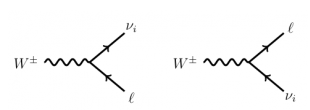
\includegraphics[width=0.6\textwidth]{W_boson.png}
\caption{Vseobecny rozpad W bosonu na leptonovy par.}
\label{sf1:fig:W_boson}
\end{figure}
\newline
Porovnanim predoslej teorie s touto dostavame, ze plati
\begin{equation}
\frac{g^2}{8M_W^2}=\frac{G_F}{\sqrt{2}}.
\end{equation}
Kedze, W bozony su nositelmi elektrickeho naboja tak je s nimi mozna aj elektromagneticke interakcia. Postup odvodenia interakcie W bosonu z fotonom si opiseme len slovne.\par
Kedze W boson je hmotna vektorova castica tak musi splnat spravanie popisane Procovym lagrangianom. V tomto lagrangiane transformujeme polia a derivacie pomocou lokalnej kalibracnej transformacie presne tak isto ako v pripade elektromagnetickej interakcie. Ked sa obmedzime na cleny, ktorych dimenzia nebude vyzsia ako 4 tak po par upravach dostaneme, ze interakcny lagrangian medzi W a fotonom ma tvar $\mathcal{L}^{em}=\mathcal{L}_{WW\gamma}+\mathcal{L}_{WW\gamma \gamma}$. Takze nas celkovy interakcny lagrangian ma tvar
$$
\mathcal{L}^{ew}=\mathcal{L}^{w}+\mathcal{L}^{em} =\mathcal{L}_{CC}+\mathcal{L}^{em}_{fermion}+\mathcal{L}_{WW\gamma}+\mathcal{L}_{WW\gamma\gamma}.
$$
Aj ked bol tento model navrhnuty, aby sa zbavil predoslych divergencii z Fermiho modelu,, pri spojeni elektrickej a slabej interakcie nam vznikli procesy, v ktorych sa objavuju dalsie divergentne cleny.\par 
Velky progres vo vyvoji prisiel, ked sa aplikovali poznatky plynuce zo studie Yang-Mills teorie zalozenu na ne-Abelovskej kalibracnej symetrii. Ukazalo sa ze tato symetria moze zrusit nejake neziaduce divergencie. Dôkladný odvodenie perturbatívnej renormalizácie zalozenu na ne-Abeliovskej kalibracnej symetrii, ktora zahŕňa Higgsov mechanizmus pre generovanie hmoty, bolo odvodene Hooft-om v roku 1971. Rozhodujúcim momentom bol experimentálny objav slabeho neutrálneho prúdu v roku 1973, ktorý jasne ukázal, ze kalibracny model, ktorý zahŕňa neutrálny vektorový bozón, moze byt pouzity na opis realneho sveta. Tento model bol nasledne vylepsovany az nakoniec dospel do tvaru, navrhnuteho Weinberg-om, Salam-om a Glashow-om, zvany ako standartny model elektroslabej interakcie. \par
Tento model je zalozeny na ne-Abelovskej SU(2)xU(1) kalibracnej grupe. Prislusnymi kalibracnymi bozonmy su 3 W bosony izospinu z SU(2) grupy ($W_1$, $W_2$, $W_3$) a B bozon slabeho-naboja z U(1) grupy. Vestky tieto polia su bezhmotne. Az ich vzajomna kombinacia bude davat uz nam zname $W^{\pm}, Z^0, \gamma$ bozony, hmotnost tymchto castic (okrem $\gamma$), vypliva zo spontanneho narusenia symetrie, ktora je zakladom tkz. Higgsovho mechanizmu, ktory je zalozeny na existencii jednej skalarnej, neutralnej a spin=0 castici - Higgsov bozon. Vyseledny lagrangian bude vo vseobecnom tvare naslednovy
\begin{equation}
\mathcal{L}_{ew}=\mathcal{L}_{K}+\mathcal{L}_{N}+\mathcal{L}_{C}+\mathcal{L}_{H}+\mathcal{L}_{HV}+\mathcal{L}_{WWV}+\mathcal{L}_{WWVV}+\mathcal{L}_{Y},
\end{equation}
kde $\mathcal{L}_{K}$ je kineticky clen pozostavajuci z  kvadratickych clenov, ktore zahrnaju dynamicke cleny a hmotnostne cleny, $\mathcal{L}_{N}$ a $\mathcal{L}_{C}$ su cleny, ktore obsahuju neutralny a nabity prud. Ich komponenty obsahuju interakcie medzi fermionmy a bozonmy, $\mathcal{L}_{H}$ obsahuje interakcne Higgs three-point and Higgs four-point self interaction, $\mathcal{L}_{HV}$ obsahuje interakcie Higgsa s W,Z bozonom, $\mathcal{L}_{WWV}$
obsahuje three-point self interakciu W,Z,$\gamma$ bozonov, $\mathcal{L}_{WWVV}$ obsahuje four-point self interakciu W,Z,$\gamma$ bozonov a $\mathcal{L}_{Y}$ obsahuje Yukawovsku interakciu medzi fermionmy a Higgsom.\par
Povedzme si teraz nejake vlastnosti a vysledky z daneho 
lagrangianu. \textbf{Unification condition} - je vztah, ktory viaze vazbove konstanty slabej interakcie a elektromagnetizmu. Moze byt vyjadrena nasledovne 
$$
e=g\sin(\theta_W)=g^,\cos(\theta_W)
$$
kde $q$ je vazbova konstanta pre SU(2) grupu, $q^,$ je vazbova konstanta pre U(1) grupu a $\theta_W$ sa vola weak mixing uhol alebo Weinbergov uhol, ktorym spontanne narusenie symetrie rotuje povodne $W_3$ a $B$ vektorove kalibracne bozony, jeho experimentalna hodnota je $\sin^2(\theta_W)=0.222\pm0.006$. Vyuzitim tohto uhla sa daju dane kalibracne polia nakonbinovat tak, ze vzniku $Z^0$ a $\gamma$ bozon. Graficky sa ta cela unification condition da znazornit nasledovne, obrazok \ref{sf1:fig:unifi}.
\begin{figure}[!h]
\centering
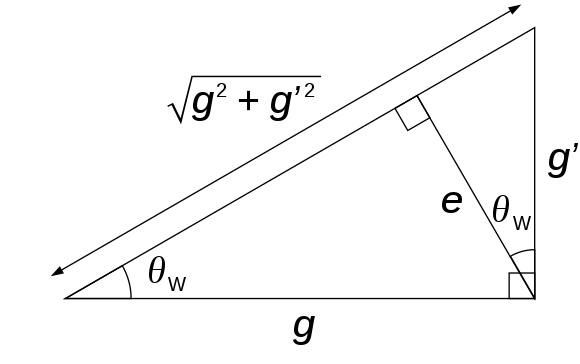
\includegraphics[width=0.6\textwidth]{Unification_condition.png}
\caption{g-vazbova kosntanta pre SU(2) grupu, $q^{,}$ je vazbova konstanta pre U(1) grupu.}
\label{sf1:fig:unifi}
\end{figure}

Hmotnosti $W^{\pm}$ a $Z^0$ sa daju vyjadrit ako 
$$
m_W=\bigg(\sqrt{\frac{\pi \alpha}{G_F\sqrt{2}}}\bigg)\frac{1}{\sin(\theta_W)}=80,42\,GeV/c^2, \hspace{0.5cm} m_Z=\frac{m_W}{cos(\theta_W)}=91.18\,GeV/c^2
$$
Uvedme základne pravidla pre konstrukciu vertexov pre slabe interakcie. V kazdom vertexe musi byt zachovavany elektrický náboj, leptonové číslo a počet kvarkov. Kedze nabité $W^{\pm}$ bozóny menia náboj kvarku, v slabých vertexoch sa nezachovávaju vône kvarkov. Ich farba ale zostava zachovaná, lebo W bozóny nie su nositeľmi farevného náboja. Je potrebne tiez zmienit, že slabé interakcie posobiace prostrednictvom W bosonov nemění generáciu leptonov. Slabé interakcie zahrnujuce W bozon sa nazyvaju interakcie nabitými prudmy, naopak slabé interakcie s Z bozonom sa nazývaju interakcie neutrálnymi prudmy. Pravidlá pre vertexy Zqq su veľmi jednoduche - nemení sa v nich leptonova generácia, kvarková vôna ani farba.\par
\textbf{Miesanie kvarkov, Cabbibov uhol, CKM matice}
Ako sme uz spominali pri odvodzovani lagrangianu v 60. rokoch minuleho storocia sa ukazali experimenty, kedy doslo k tomu, ze sa nezachovavala podivnost. Tie su sice potlacene oproti tym, co nemenia podivnost ale aj tak existuju a to bolo treba vysvetlit a popisat. S popisom prisiel Gabibbo, ktory si vsimol pozoruhodne suvislosti medzi znamymi slabymi procesmy. Pre procesy kde sa podivnost nemeni ma efektivna hadronova konstanta hodnotu $G_F\cos(\theta_C)$, pre podivnost meniace procesy ma tato efektivna konstanta hodnotu $G_F\sin(\theta_C)$. Experimentalne sa urcilo, ze Gabibbov uhol ma hodnotu $\theta_C=13.04^{\circ}$. V ramci dvojgeneracneho modelu (u, s, d, c kvarky) je mozne take zmiesavanie popisat pomocou realnych koeficientov, ktore je mozne suhrnne zapisat do tvaru matice
\[ U_C=
\begin{pmatrix}
    \cos(\theta_C) & \sin(\theta_C) \\
    -\sin(\theta_C) & \cos(\theta_C) \\
\end{pmatrix}=
\begin{pmatrix}
    U_{ud} & U_{us} \\
    U_{cd} & U_{cs} \\
\end{pmatrix}
\]
tato matica popisuje zmiesavanie kvarkov, ktore sa da napisat nasledovne 
\[
\begin{pmatrix}
    \bar{u},\bar{c} \\
\end{pmatrix}=
\begin{pmatrix}
    \cos(\theta_C) & \sin(\theta_C) \\
    -\sin(\theta_C) & \cos(\theta_C) \\
\end{pmatrix}
\begin{pmatrix}
    d \\
    s \\
\end{pmatrix}
\]
Pre tri generacie je zmiesavanie kvarkov vyjadrene pomocou Cabibbo-Kobayashi-Maskawovou maticou
\[ V_{CKM}=
\begin{pmatrix}
    V_{ud} & V_{us} & V_{ub} \\
    V_{cd} & V_{cs} & V_{cb} \\
    V_{td} & V_{ts} & V_{tb} \\
\end{pmatrix}
\]
jej elementy su obecne komplexne (daju sa parametrizovat pomocou troch uhlov Gabibbovho typu a jednou fazou). Presne vyjadrenie elementov CKM matice patri k hlavnym aktualnym cielom experimentalnej casticovej fyziky lebo predstavuje jeden zo zasadnych testov spravnosti Standartneho modelu elektroslabej interakcie.
\[
\begin{pmatrix}
    \bar{u} & \bar{c} & \bar{t} \\
\end{pmatrix} 
\begin{pmatrix}
    0.975 & 0.221 & 0.022 \\
    0.221 & 0.974 & 0.040 \\
    0.009 & 0.039 & 0.999 \\
\end{pmatrix}
\begin{pmatrix}
    d \\
    s \\
    b \\
\end{pmatrix}
\]
Hodnoty CKM matice na diagonale su skoro rovnake velke a blizko jednotky co implikuje napriklad, ze $t$ kvark sa s najvacsiou pravdepodobnostou rozpadne na $b$ kvark. Nediagonalne prvy su zase dost male.\par Obecne plati, ze kvark s nabojom $+2/3$ (u, c, t) sa transformuje na kvark s nabojom $-1/3$ (d, s, b) a naopak prostrednictvom nabiteho $W^{\pm}$ bozonu, ktory meni naboj o jednotku. Tiez plati, ze sa kvarky rozpadaju v postupnosti od najviac hmotnych po tie najmenej hmotne 
$$
t\rightarrow b\rightarrow s\rightarrow u \leftrightarrow d
$$
Nasledujuci obrazok graficky znazornuje prechody medzi kvarkmy \ref{sf1:fig:Kvarky_prechody}
\begin{figure}[!h]
\centering
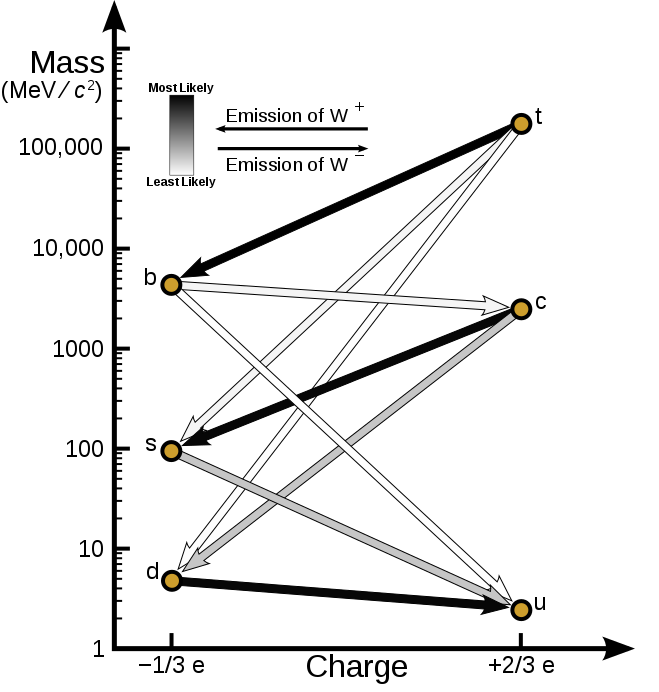
\includegraphics[width=0.6\textwidth]{Kvarky_prechody.png}
\caption{Diagram znazornujuci prechodove moznosti medzi kvarkmy prostrednictvom slabej interakcie a indikacie pravdepodobnosti prechodov, ktore su dane CKM maticou.}
\caption{}
\label{sf1:fig:Kvarky_prechody}
\end{figure}

\subsection{Silná interakcia}
Silna interkcia je sila posobiaca len medzi casticami s nenulovym \textcolor{red}{fa}\textcolor{green}{reb}\textcolor{blue}{nym} nabojom, ktory obsahuju iba kvarky a nie je preto univerzalna interakcia. Je silna len na malych vzdialenostiach hadronov a jej dosah je priblizne $10^{-15}\,m$. Jej prejavmy su 
\begin{itemize}
	\item jadrove sily medzi nukleonmy v jadre  
	\item sily, ktore drzia kvarky pohromade v nukleone
	\item produkcia castic pri vysokoenergetickych zrazkach jadronov
\end{itemize}
Okrem toho, ze silna interakcia nie je univerzalna, cize plati len pre kvarky, tak je aj obmedzena vacsim poctom zakonov zachovania ako ostatne interakcie.\par
Silnej interakcii prislucha vazbova konstanta, ktora charakterizuje jej velkost
$$
\alpha_s= \frac{g_s^2}{4\pi},
$$
kde $g_s$ je naboj konstituentneho kvarku. Pre male energie je hodnota tejto konstanty $\alpha\approx 1$. Vazbova konstanta pre silnu interakciu je ovela vacsia ako pre elektromagneticku interakciu. Velkost tejto konstanty pre male energie ma za nasledok nepouzitelnost poruchovej teorie kvoli divergentnym clenom. Avsak tato konstanta ma tu vlastnost, ze jej velkost zavisi od prenesenej energie (resp. hybnosti), preto sa tato konstanta nazyva aj $beziaca$ vezbova konstanta. S rastucou energiou interakcie (s rastucou hybnostou zrazajucich sa castic) totiz tato vazbova konstanta klesa, co vedie k asymptotickej volnosti (divergentne cleny zacnu konvergovat, co umozni pouzit poruchovu teoriu). Zavislost $\alpha_s$ na hybnosti je nasledujuca
$$
\alpha_s\approx\frac{12\pi}{(11n_c-2n_f)\ln\big(\frac{k^2}{\Lambda^2}\big)}
$$ 
kde $n_c$ je pocet farebnych nabojov, $n_f$ je pocet kvarkovych druhov castice (flavour) a $\Lambda$ je skalovaci parameter vychadzajuci z renormalizacneho procesu a ma hodnotu priblizne $200\,MeV$. (Napr. $\alpha_s=0.12$ pre $k^2=(100\,GeV)^2$.)\par
Mediatorom silnej interakcie je vektorova castica gluon, ktora je neutralna a nehmotna, nieco ako foton pre QED. Avsak pre elktromagneticku interakciu mame len dva typy elektrickeho naboja: kladny a zaporny. V teorii silnej interakcie, ktora je popisana kvantovou chromodynamikou (QCD), vsak existuje 6 druhov naboja, ktory sa z nevysvetlitelnej priciny nazyvaju \textcolor{red}{fa}\textcolor{green}{reb}\textcolor{blue}{ny} naboj a su to tieto, obrazok \ref{sf1:fig:Color_quarks}
\begin{figure}[!h]
\centering
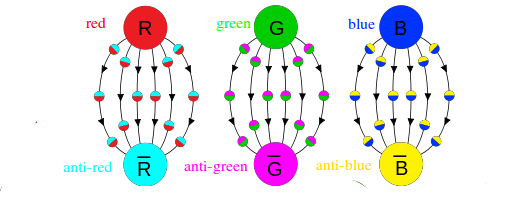
\includegraphics[width=0.6\textwidth]{Color_quarks.png}
\caption{6 druhov kvarkov, horne tri su farebne naboje red, green, blue a spodne su ich anti-farebne naboje anti-red, anti-green, anti-blue.}
\label{sf1:fig:Color_quarks}
\end{figure}
\newline
Podla QCD su baryony (castice tvorene z 3 kvarkov) a mezony (castice tvorene jednym kvarkom a anti-kvarkom) farebne neutralne. Pre glouny plati, ze su nositelmy aj jednej farby aj jednej anti-farby sucasne, kebyze to tak nie tak by potom hadrony nemohli byt viazane vo farebne neutralnom systeme.  Z toho potom mame celkovo $3^2=9$ moznych farebnych kombinacii pre gluony. Avsak ako vieme, nie je to uplne pravda, ze ich je 9. V skutocnosti mame len 8 gluonov a to z toho dovodu, ze bezfarebny singletny stav $\frac{1}{\sqrt{3}}(r\bar{r}+b\bar{b}+q\bar{q})$, nesprostredkovava ziadnu interakciu medzi farebnymi stavmy. Moze nanajvys interagovat s dalsim singletnym stavom. Avsak interakcie s gluónmi na dlhé vzdialenosti neexistujú, čo dokazuje, že ani gluóny v singulárnom stave neexistujú.\par
Podme si nacrtnut ako to v takom bezfarebnom systeme vlastne funguje. Majme nasledujuci obrazok \ref{sf1:fig:Prechody}
\begin{figure}[!h]
\centering
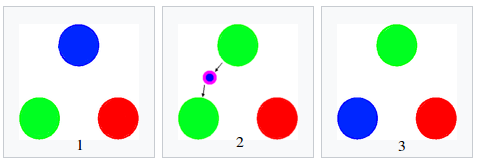
\includegraphics[width=0.8\textwidth]{Color_changing.png}
\caption{}
\label{sf1:fig:Prechody}
\end{figure}
\newline
Na 1. obrazku mame system ktory je bezfarebny a zatial neprebieha ziadna vymena gluonu. Na 2. obrazku vsak uz mame gluon, ktory sa uvolnil z modreho kvarku. Kedze tento gluon pochadza z modreho kvarku tak jeho farebna polovica musi byt modra. Ta anti-farebna cast gluonu moze byt prakticky hocijaka. V nasom pripade je anti-zelena. Kedze sa odnasa anti-zelena farba tak kvark musi byt zeleny aby bol cely system stale farebne neutralny. Na 3. obrazku sa gluon obsarboval do zeleneho kvarku. Tam sa spolocne vybili anti-zelena a zelena farba a jedine co z gluonu ostalo je modra farba. Navyse gluony maju tu vlastnost, ze mozu interagovat medzi sebou, to fotony napriklad nemozu. Takze, ked mame system, kde je viacej gluonov, moze dojst k tomu, ze gluony navzjom budu interagovat, co moze viest k tomu, ze sa zmeni ich celkovy farebny naboj. Avsak stale sa nesmie zmenit celkovy farebny naboj systemu. Pre nazornejsie a krajsie vysvetlenie odporucam si pozriet toto video (Introduction to subatomic physics and subatomic particles: Part III na YOUTUBE).\par
Vzhladom k tomu, ze su gluony nehmotne je mozne ocakavat, ze cast statickeho QCD potencialu bude podobna QED potencialu. Tvar QCD potencialu je 
$$
V_{QCD}=-\frac{4}{3}\frac{\alpha_s}{r}+kr.
$$ 
Tento potenacial sa nazyva Cornell-ov potencial. Faktor $4/3$ vyplyva z toho, ze mame 8 farebnych gluonov, ktore moze posobit na 3 kvarky o roznych farbach. Vidime, ze pre male hodnoty $r$ dominuje negativna cast potencialu a nastava \textit{assymtotic freedom} a mozme pouzit one-gluon exchange (to je vlastne len to, ze mozme pocitat poruchovu teoriu s predpokladom, ze sa tam vymiena gluon, podobne nieco ako pre foton ked sa vymiena). Druhy clen je asociovany s viazanostou kvarkou. Pre velke vzdialenosti je potencialna energia medzi kvarky taka velka, ze v istom momente sa tato energia premeni na novo vzniknuty kvark-antikvark par. Takze namiesto toho, aby sme dostali oddeleny kvark a anti-kvark, dostaneme dva pary kvark-antikvark.\par
Vertex faktor silnej interakcie pozostava z kvarkov a gluonov. Zakladny vertex sa sklada z dvoch fermionovych liniek a jednej bozonovej. Ako sme uz spominali vysie, na rozdiel od QED je mozne v tomto pripade mat aj dva vertexy, ktore zahrnuju troj- a stvor- gluonovu interakciu. Toto je zakladny rozdiel oproti QED, kde fotony navzajom medzi sebou neinteraguju. Vyskyt z tychto vertexov v QCD je mozny vdaka ne-Abelovskej kalibracnej transformacii. Je to velmi podobne tomu, co sme mali pre elektroslabu interakciu. Aj tam sa totiz nachadzaju pripady, kedy dochadza ku troj- a stvor- bozonovej interakcii, ktora je taktiez podmienena touto ne-Abelovskou kalibracnou transformaciou. Akurat tam medzi sebou interaguju $W^{\pm}, Z^0$ a $ \gamma$ bozony. Porzi nasledujuci obrazok \ref{sf1:ref:vertexy}.
\begin{figure}[!h]
\centering
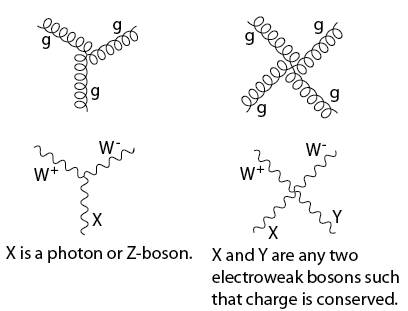
\includegraphics[width=0.5\textwidth]{Vertexy.png}
\caption{}
\label{sf1:ref:vertexy}
\end{figure}
\newline
Kedze sme sa uz dostali k tym kalibracnym transformaciam, zadefinujme si, co to ta QCD vlastne je. QCD je typ kvantovej teórie poľa zvanej teória ne-Abelovskej kalibracnej transformacii so skupinou symetrií SU(3) navrhnuta David-om Gross-om, David-om Politzer-om, and Frank-ok Wilczek-ok . Lgrangian pre 
QCD ma tvar
\begin{equation}
\begin{gathered}
\mathcal{L}_{QCD}=-\frac{1}{4}G^a_{\mu\nu}G^{a\mu\nu}+
\sum_{\psi}\bar{\psi}_i\big(i\gamma^{\mu}(\partial_{\mu}\delta_{ij}-ig_sG_{\mu}^aT_{ij}^a)-m_{\psi}\delta_{ij}\big)\psi_j\\
G_{\mu\nu}=\partial^{\mu}A^{\nu}-\partial^{\nu}A^{\mu}+gf_{abc}A^{\mu}_bA_c^{\nu}
\end{gathered}
\end{equation}
kde $G^{\mu\nu}$ je antisymetricky tenzor, ktoreho posledny clen kompenzuje nekomutativnost rotacii vo farebnom priestore, a tento posledny clen moze za tu troj- a stvor- gluonovu self-interakciu, $\psi_i$ je Dirakov spinor kvarkoveho pola s farbou i=(r,q,b), $G_{\mu}^a$ je 8 komponentne SU(3) kalibracne pole, $T_{ij}^a$ reprezentuje 3x3 Gell-Mannovu maticu, $g_s$ silna vazbova konstanta.\par
Existuje vela sposobov ako nalozit s QCD. Da sa k nej pristupovat pomocou poruchovej teorie, ktora je zalozena na assymptotickej volnosti (male $\alpha_s$). Medzi neporuchovýma teoriema ma najsilnejsie postavenie tkz. Lattice QCD - k redukcii analytickych integrabilnych drahovych integralov sa na numericke vypocty poziva sada diskretnych bodov rozlozenych na mriezke (lattice). Pre riesenie specifickych problemov sa pouzivaju efektivne teorie, ktore v istych limitach davaju kvalitativne presne vysledky. Takouto teoriou je napriklad Chiralna poruchova teoria, co je efektivna teoria pre QCD pri nizkych energiach.\par
\textbf{Hadronizacia} alebo tiez fragmentacia je formovanie hadronov z kvarkov a gluonov. Tento jav moze nastat po vysoko-energetickych zrazkach v collideri castic, kde su produkovane "volne" kvarky a gluony. Takato produkcia parov moze vzniknut napriklad anihilaciou pri interakcii $e^-e^+$. Nasledne medzi kvarkom a antikvarkom nastava dynamicka separacia. Ta nastane preto, lebo tieto castice maju taku velku energiu, ze sila, ktora ich drzi po kope nie je dostatocne velka, aby tomu zabranila. Su dva pristupy ako kvantitativne pochopit proces formovania hadronov: 
\begin{itemize}
	\item Chromostatic \newline
	Kvark-antikvark par vytvori dalsi kvark-antikvark par, akonahle vzdialenost medzi prvym povodnym parom je radovo $1\,fm$. Pri takejto vzdialenosti je hustota energia medzi kvarkmy natolko velka, ze dojde k vytvoreniu dalsieho paru. Tento proces pokracuje az kym relativna hybnost kvarkov neklesne na taku hodnotu, ze uz nebude moct dochadzat k tvoreniu dalsich parov, pozri obrazok \ref{sf1:fig:anihilation}. Hadrony nasledne vznikaju pozdlz retazca tvorenia kvarkov. Vytvorene hadrony produkuju sprsku zvanu jety, ktore su priblizne v smere prveho kvarku, anti-kvarku.
	\begin{figure}[!h]
	\centering
	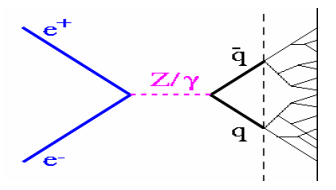
\includegraphics[width=0.3\textwidth]{Anihilation.png}
	\caption{}
	\label{sf1:fig:anihilation}
	\end{figure}
	\item Chromodynamical \newline
	Tento pristup sa odohrava tkz. kvark-gluonovou kaskadou, pozri obrazok \ref{sf1:fig:cascade}. Zacina emisiou gluonu kvarkom alebo anti-kvarkom. Tento gluon moze produkovat bud kvark-antikvark par alebo gluonovy par. Kedze je viacej gluonov ako kvarkov tak statisticky sa tento gluon bude rozpadat viacej do gluonov ako do kvarkov. Silna vazba bude narastat so zmensujucou sa hodnotou hybnosti virtualnej castice. Na konci kaskady kvarky vytvoria bezfarebne viazane stavy. Je jasne, ze tento model nemoze byt pouzity az na koniec hadronizacneho procesu. Dovodom je, ze pre male hodnoty hybnosti sa vazbova konstanta zvacsuje a tym sa narusa poruchovy rozvoj. V tejto oblasti prevláda elasticky efekt, ktorý skončí tvorbou hadronou. Hadrony su tvorene vo vakuu na konci kvark-gluonovej kaskady. Transverzalna hybnost hadronov vzhladom na povodny smer kvarkuje je limitovana Heisenbergovym principom neurcitosti. Hadrony su preto koncentrovane okolo povodneho smeru kvarku a tvoria jety. Ak ma prvy gluon dostatocne velku transverzalnu hybnost, tak moze vzniknut treti hadronovy jet v smere tohto gluonu.
	\begin{figure}[!h]
	\centering
	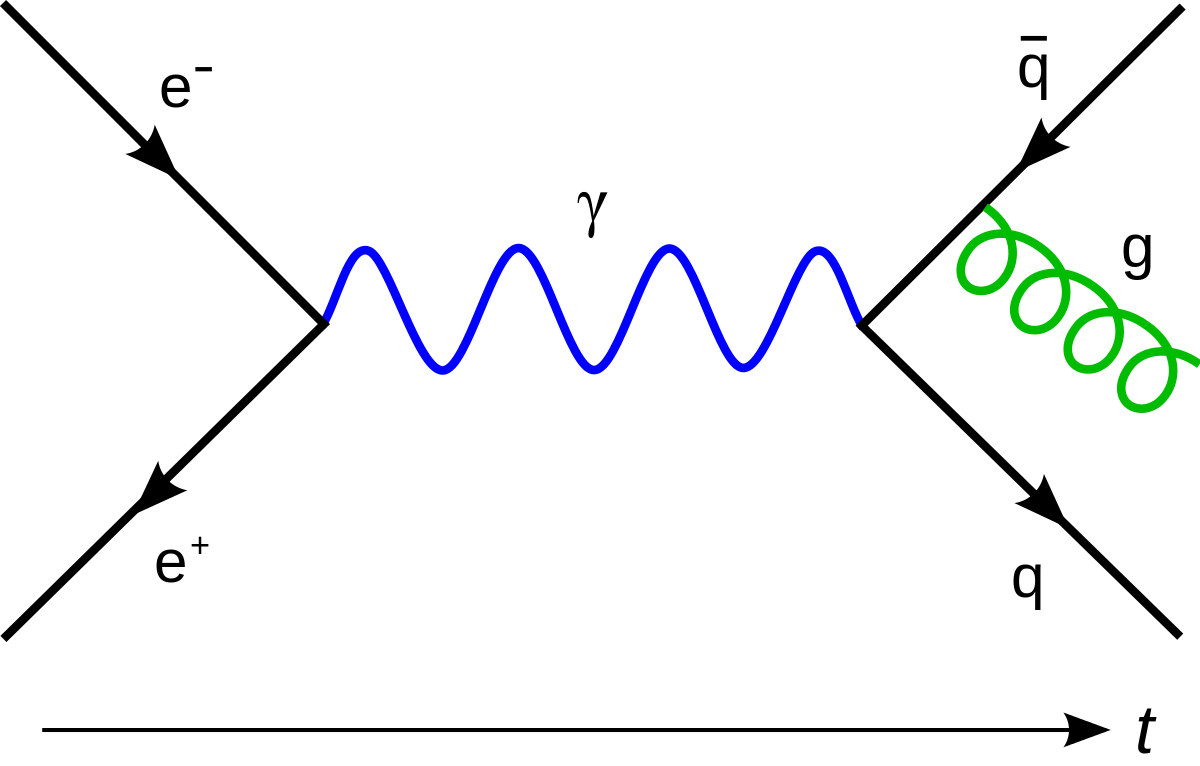
\includegraphics[width=0.3\textwidth]{Cascade.png}
	\caption{}
	\label{sf1:fig:cascade}
	\end{figure}
\end{itemize}
\par
Dynamika tychto hadronizacnych procesov stale nie je uplne pochopena pomocou QCD a to vdaka tomu, ze poruchova teoria v QCD, formulovana pomocou kvarkov a gluonov, je platna len na malych vzdialenostiach. Na vacsich vzdialenostiach sa tato poruchova teoria zhrouti. Existuju vsak rozne fenomenologicke modely, ktore sa to snazia popisat. Prvym takymto modelom bol Feynmanov a Fieldov, nezavisle vytvoreny, fragmentacny model. Zakladnou myslienkou tohto modelu je predstava hodronizacie kvark-dikvarkoveho systemu ako nezavislej fragmentacie kvarku a dikvarku. Tento predpoklad je ale v principe neudrzatelny, pretoze k hadronizacii dochadza vdaka vzajomnej interakcii medzi nimi. Avsak ukazalo sa, ze vysledne rozdelenie hadronov moze byt v istom priblizeni popisane fragmentacnou funkciou $D^h_q(k,p_T)$ (jazyk fragmentacneho modelu). Ta popisuje pravdepodobnost, ze parton $q$ vytvori hadron $h$ nesuci cast $k$ z povodnehej energie partonu a pricnou hybnostou $p_T$. Tato funkcia ako kazda ina distribucna funkcia by mala byt univerzalna t.j. nezavisla na procese. \par
\textbf{Jet} je sprska castic, ktora sa nachadza v uzkom kuzely, ktora vznika pri hadronizacii kvarkov a gluonov. Su to vlastne experimentalne znaky kvarkov a glunov produkovanych vo vysoko-energetickej fyzike, pozri obrazok \ref{sf1:fig:jet}. 
\begin{figure}[!h]
\centering
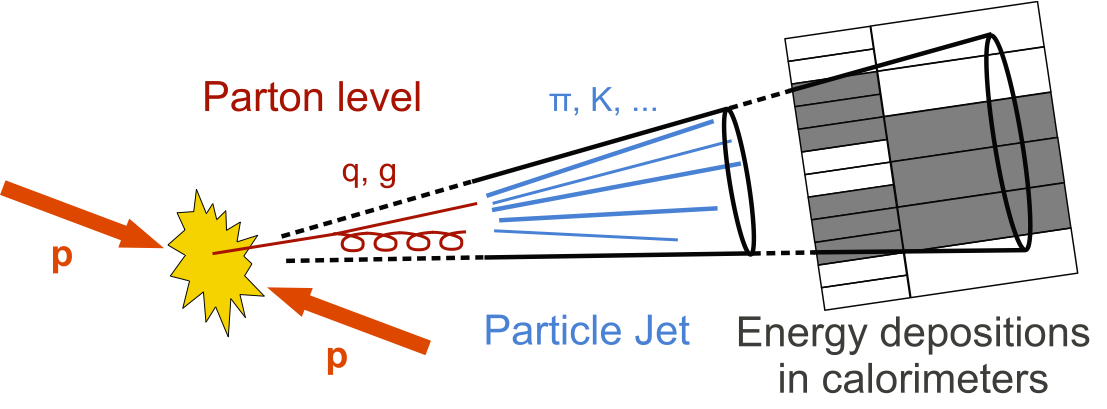
\includegraphics[width=0.7\textwidth]{Jet.png}
\caption{}
\label{sf1:fig:jet}
\end{figure}
Skutocnost, ze smery a energie jetov dobre odpovedaju smerom a energiam povodnych kvarkov, nie je triavalna vlastnost procesu hadronizacie. Smerove rozdelenie jetov v priestore vzhladom ku smeru $e^-e^+$ zrazky by malo byt rovnake ako koncovy stav pri procese $e^-e^+\rightarrow \mu^-\mu^+$, pretoze miony a kvarky maju spin 1/2. Tento fakt je jednym zo silnejsich dokazov toho, ze kvarky maju spin 1/2. Kvark, anti-kvark a gluon mozu fragmentovat do hadronov, co vedie ku troj-jetovym eventom. Vzhladom k tomu, ze uhlove rozdelenie jetov je v sulade s teoretickou predpovedou pre gluon so spinom 1, poskytly tieto eventy jednoznacny dokaz o existencii gluonov.
\subsection{Gravitačná interakcia}
Tato sila sa uplatnuje len pri silovom posobeni medzi makroskopickymi objektmy a v kozmickej mechanike. V subatomarnej fyzike nehra podstatnu rolu a preto moze byt zanedbana. Starsia teoria gravitacie pochadza od Newtona, ktory tuto silu popisal ako $$ \vec{F}=\kappa\frac{m_1m_2}{r^2}\frac{\vec{r}}{r}, $$ kde $\kappa=6.672\times10^-11\,m^3kg^-1s^2$, je vazbova konstanta. Jej posobenie je nekonecne, podobne ako pre elektromagneticku interakciu. Da sa povedat, ze to je najdemokratickejsia sila aku pozname. Pretoze je univerzalna a na vsetky telesa posobi rovnako. Modernou teoriu gravitacie je Vseobecna teoria relativity, ktora tvrdi, ze zrychlenie a gravitacna sila je ta ista vec. Sprostredkovatelom tejto interakcie je graviton (zatial nebol pozorovany), ktory by mal byt nehmotny a mal by mat spin=2.
\section{Vlastnosti leptónov a hadrónov}
Sem si pripomenieme vlastnosti, ktore sme hore neuviedli.
A ak spomiem nieco tak to je dolezite a je dobre si to znovu pripomenut.\newline
\textbf{Leptony}
\begin{itemize}

\item Leptony nemaju farebny naboj a tak nepodliehaju silnej interakcii podobne ako neutrina, ktore nemaju elektricky naboj a tak nepodliehaju elektromagnetickej interakcii. Neutrina interaguju jedine slabo.
\item Kedze leptony maju spin, mozu vytvarat magneticke pole. Velkost magnetickeho dipoloveho momentu je dany 
$$\mu=g\frac{Q\hbar}{4m},$$ kde $m$ je hmotnost leptonu, $g$ je tkz. g-faktor pre lepton. Prvy rad pribliznej kvantovej mechaniky predpoveda tuto hodnotu rovnu 2 pre vsetky leptony. Avsak, vyzsie rady kvantoveho efektu sposobuju korekciu tejto hodnoty oznacovanu ako anomalny magneticky moment. Toto cislo je velmi citlive na vela detailov a preto jeho spocitanie a nasledne experimentalne zmeranie bolo obravskym uspechodm QED. Vo Feynmanovych diagramoch toto cislo reprezentuju slucky. Tato korekcia ma priblizne hodnotu $a_e=0.001159....$ 
\item vsetky leptony, okrem tau neutrina, boli pozorovane priamo v experimentoch - ako volne castice.
\item Presne merania mionovych vlastnosti boli vykonane prostrednictvom skumania mezoatomov vytvorenych zachytenim mionu v atomu na Bohrove orbite. Hodnota energie stavu mezoatomu s hlavnym kvantovym cislom $n$ je linearne umerna hmotnosti mionu$$E(n)=-\frac{Z^2e^4m}{2(4\pi\epsilon_0)^2\hbar^2n^2}$$ a teda je v absolutnej hodnote asi 200-krat vacsia nez energie odpovedajuce tomu istemu stavu ale s elektronom. Prechod do stavu z nizsou hladinou energie sposobuje emisiu rentgenoveho ziarenia, ktore je charakteristicke a mozno z neho vyvodit informacie o naboji, hmotnosti a spine.
\item Doba zivota mionov je okolo $\tau_0=2.2\mu s$ a ich rychlost je $\beta=0.98$. Velka cast mionov vznika vysoko v atmosfere, asi 10km nad zemou. Kedze sa pohybuju tak rychlo nastava dilatacia casu vzhladom na pozorovatela na Zemi. To znamena, ze vo svojej sustame ma mion dobu zivota tych $\tau_0$ ale v sustave pozorovatela, ktory stoji na zemskom povrchu a sleduje miony je ten cas o cosi dlhsi presnejsie $\tau=\tau_0/\sqrt{1-\beta^2}\approx11\mu s$. Takze drahu, ktoru prejde mion urcime velmi jednoducho  $l=\beta c\tau \approx 13.2\,km$. A preto je mozne, ze pozorujeme kozmicke miony na povrchu Zeme. Toto je aj jeden z dokazov Einsteinovej teorie relativity.
\item dominantny rozpad mionu: $\mu^-=e^-+\bar{\nu}_{e^-}+\nu_{{\mu}^-}$. Ostatne mozne rozpady např. $\mu^-=e^-+\gamma$ je sice kinematicky mozny ale nezachovava sa flavor number. Taketo rozpady maju $BR\sim10^{-12}$.
\item Helicita částice je vyjadrenie orientacie medzi spinom castice a jej hybnostou. Castice, ktorych spin je orientovany v rovnakom smere ako hybnost, su pravo-tocive a v pripade, ze orientacia je v protismere tak hovorime o lavo-tocivych casticiach. Pre QCD a QED su castice rovnako pravo a lavo tocive, nedochadza tam k ziadnej asymetrii. Avsak, v pripade slabej interakcie mame len lavo-tocive fermiony a pravo-tocive neutrina-maximalne narusenie parity.
\item Elektricky naboj moze byt spocitany z projekcie spinu a slabeho-hypernaboja cez $Gell-Mann-Nishijima$ formulu $$Q=T_3+\frac{Y_W}{2}$$.
\item Kineticka energia $\beta$ castica ma spojite spektrum od 0 az po maximalnu predanu energiu. Typicka energia je $1\,MeV$, ale extremnych pripadoch to moze byt aj niekolko $10\,MeV$. Fundamentalny $\beta$ rozpad nastava vdaka konverzii d-kvarku nautronu na u-kvark protonu emisiou $W^-$ bozonu, ktory sa nasledne rozpada na $e^-$ a $\nu_{e^-}$.
\item $\Gamma\sim KG_F^2m_l^5$, kde $K$ je ciselna konstanta, $G_F$ je Fermiho konstanta a $m_l$ je hmostnost leptonu. Stredna doba zivota je $\tau=\hbar/\Gamma$
\item Kvarky, ktore urcuju vlastnosti hadronov sa nazyvaju valencne kvarky. Hadrony naviac obsahuju tiez prchave kvark-antikvark pary, ktore nemenia vlastnosti, ale prispievaju k jeho kludovej energii. Tieto kvarky sa nazyvaju morske kvarky.
\item $$ R=\frac{\sigma(e^+e^-\rightarrow q\bar{q})}{e^+e^-\rightarrow \mu^+ \mu^-}=3\Sigma_{q}e^2_q$$ tento pomer je zalozeny na tom, ze existuju tri farebne stavy kvarkov a je na energii takmer nezavisly. Porovnanim experimentach dat vychadza, ze to sedi.\newline
\end{itemize}
\textbf{Hadrony}
\begin{itemize}
	\item Vlastnosti hadronov ako naboj, spin, atd. su urcene valencnymi kvarkmy, zatialco hmotnost hadronov ma s valencnymi kvarkmy velmi malo spolocne a velka cast hmotnosti pochadza z mnozstva energie, ktoru prenasaju gluony.
	\item Hadrony sa rychlo rozpadaju silnou interakciou, pokial im to umoznia kvantove cisla (zakony zachovania kvantovych cisiel). Dalej potom uz pracuje slaba interakcia, ktora meni vonu kvarkov az na kvarky prvej generacie a nakoniec az na nejake leptony.
	\item Najtazsie zname castice, vznikajucí pri casticovych interakciach pri vysokych energiach, su hadrony zvane hyperony. Vsetky hyperony vykazuju silnu interakciu a su vysoko nestabilne s velmi kratkou dobou zivota. Vzhladom k tomu, ze hyperony interaguju silno, mozu vstupovat do jadier a byt tam naviazane jadrovymi silami - vzniknu hyperjadra. V typickom hyperjadre je jeden nukleon nahradeni hyperonom. Su to nestabilne utvary, ktore sa rozpadaju dvojako: bud mezonovym rozpadom alebo nukleonovym rozpadom.
	\item Hypernaboj je definovany ako $Y=B+S+C+T+\tilde{B}$, kde jednotlive znaky su baryonove cislo, podivnost, povab, topness a beauty - kvantove cisla. Nasledne vdaka tomu mozme spocitat priemet izospinu $I_3=Q-Y/2$, kde $Q$ je elektricky naboj.
\end{itemize}
\section{Symetrie a zákony zachovania}
\textbf{Izospin}\par
Fyzikální veličina, kterou zavedl v roce 1935 Eugene Paul Wigner, aby mohl popsat multiplety různých částic. Jedná se o kvantové číslo související se silnou interakcí. Částice, na něž působí silná interakce shodně, ale které mají různý elektrický náboj, lze považovat za jedinou částici s hodnotou izospinu související s počtem nabitých stavů. Izospin je bezrozměrná veličina a její název je odvozen od skutečnosti, že matematické struktury, které popisuje, jsou podobné těm, které popisuje vnitřní moment hybnosti, zvaný spin.\par
Některé částice mají mnoho společných znaků, proto je možné chápat je jako obměny jediného objektu. K rozlišení těchto stavů se zavádějí různá kvantová čísla, z nichž nejčastější je izospin. Takové skupiny příbuzných elementárních částic se nazývají multiplety. Částice v multipletu se vzájemně liší projekcí izospinu. Všechny částice multipletu mají stejnou velikost izospinu a liší se její projekcí do libovolné osy, pozri obrazok \ref{sf1:fig:Baryon_decuplet}.\par
\begin{figure}[!h]
\centering
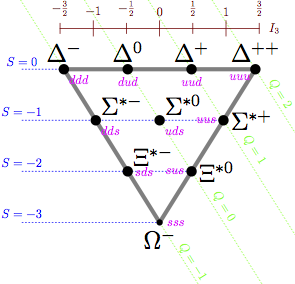
\includegraphics[width=0.5\textwidth]{Baryon_decuplet.png}
\caption{Kombinácia troch u, d alebo s-kvarkov tvoriacich baryóny so spinom=3/2 tvorí baryónový decuplet.}
\label{sf1:fig:Baryon_decuplet}
\end{figure}
Částice v rámci jednoho multipletu se od sebe odlišují převážně elektrickým nábojem, popsaným zetovou složkou izospinu. Naopak příbuzné částice v multipletu mají stejnou hodnotu spinu, baryonového čísla a podobnou klidovou hmotnost.\par
Zjistilo se, že při procesech způsobovaných silnou interakcí se hodnota izospinu zachovává, zatímco v procesech elektromagnetické interakce se hodnota izospinu může zvýšit nebo snížit o jedničku.\par
Počet částic v multipletu je dán hodnotou izospinu. Kupříkladu pro nukleon je hodnota izospinu 1/2, multiplet má tedy dvě částice neutron a proton a nazýváme ho dublet. Je-li hodnota izospinu 1, má multiplet 3 částice, příkladem může být kladný, záporný a neutrální pion, takový multiplet nazýváme triplet. Existují též singlety, pro ně je izospin roven 0. Příbuzné částice v multipletu, například proton a neutron, lze považovat za různé kvantové stavy jediné částice = nukleon. Izospin tyto částice odlišuje.\newline
\textbf{Dalsie hadronove cisla}\par
Vedla izospinu je tu este sada kvantovych cisiel, ktore su charakteristicke len pre hadrony. Su to baryonove cislo B, podivnost S, povab C, krasa B, topness T. 


Obrazok \ref{sf1:fig:zzachovania} znazornuje veliciny a ich zachovavanie sa v roznych interakciach. 
\begin{figure}[!h]
\centering
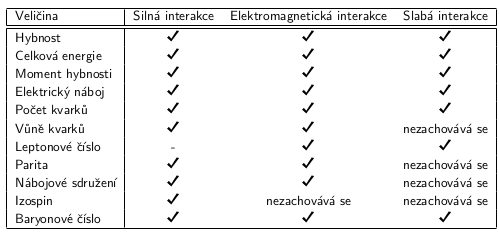
\includegraphics[width=0.9\textwidth]{Zakony_zachovania.png}
\caption{Tu len pripomeniem, ze baryonove cislo je definovane ako $B=\frac{1}{3}(n_q+n_{\bar{q}})$. Pre leptonove cislo plati $L=n_l-n_{\bar{l}}$, tu musi byt zachovany aj flavor leptonu. Napriklad takyto proces nie je pozorovany: $\mu^- \rightarrow e^-+\gamma$.}
\label{sf1:fig:zzachovania}
\end{figure}
\newline
Skor ako prejdeme ku samotnym zakonom vysvetlime najprv vyznam zakonu zachovania. So zakonmy zachovania velmi suvisia transformacie. Predpokladajme, ze mame system popisany lubovolnymi suradnicami, napr. $\vec{r}=x,y,z.$ Nasledne posunieme system po osi $x$ o vzdialenost $a$. Prepokladajme, ze fyzikalny popis systemu sa tymto nezmeni, tzn. chovanie systemu je invariantne voci pousnutiu pozdlz osi $x$.\par
V teoretickej fyzike existuje teorem, ktory spojuje invarianciu vzhladom k danej transformacii so zachovavajucou sa velicinou-\textbf{Noetherovej teorem}: Kazdej grupe transformacii suradnic zavislych spojito na realnom parametri, pri ktorych Lagrangeova funkcia zostava invariantna, odpoveda prvy integral Lagrangeovych rovnic tejto sustavy $=$ zakon zachovania. V nasom pripade invariancia vzhladom k posunutiu v $x$-ovej osi sa teda dostaneme k zachovaniu $x$-ovej zlozky hybnosti. Tato invariancia sa nazyva symetria systemu.\par 
Uvedieme zhrnutie, obrazok \ref{sf1:fig:zzachovania}, tychto spojitych transformacii a k nim pridruzime zachovavjuce sa veliciny za predpokladu, ze system je invariantny voci danym transformaciam
\begin{figure}[!h]
\centering
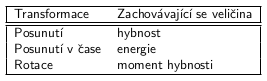
\includegraphics[width=0.5\textwidth]{spojite_trans.png}
\caption{Spojite transformacie a s nimi spojene zachovavajuce sa veliciny. Vsetky spojite transformacaie su spojene s aditivnymi kvantovymi cislamy, aditivne v tom zmysle, ze vsetky prispevky roznych casti systemu sa scitaju do celkovej hodnoty.}
\label{sf1:fig:spojtran}
\end{figure}
\newline
Spojite transformacie maju tu vlastnost, ze kazda transformacia moze byt vyjadrena ako sucet malych transformacii. Opakom k tymto transformaciam su transformacie diskretne, ktore nemoze byt vyjadrene pomocou mensich transformacii. Medzi diskretne veliciny patri Parita, Nabojove zdruzenie alebo Time reversal.\newline

\textbf{Parita} \par
Pred rokom 1956 fyzici verili, ze zrkadlovy obraz akehokolvek fyzikalneho procesu reprezentuje dalsi mozny fyzikalny proces. A prave v tomto roku bol Lee-om a Yang-om navrhnuty experimentalny test, ktory mal zistit ci je to pravda, a to aj pri posobeni slabej interakcie. V tomto experimentu boli poctivo zrovnane spiny jadier $^{60}Co$ tak, aby mierili vsetky do jedneho smeru (povedzme, ze napriklad hore). Kobalt sa nasledne rozpadol beta rozpadom a bol pozorovany smer vyletujucich elektronov. Tento smer pre podstatnu vacsinu elektronov bol v smere spinu jadier kobaltu.\par 
Toto jednoduche pozorovanie malo vsak udivujuce nasledky. Predpokladajme, ze pozorujeme zrkadlovy obraz tohto procesu. Obraz jadra rotuje opacnym smerom (spin smeruje dolu). Zrkadlove elektrony ale aj tak vylietavaju smerom hore, ako to bolo v predchadzajucom pripade. V zrkadlovom odraze su tak elektrony emitovane v smere opacnom k smeru spinu jadier. Mame tak fyzikalny proces, ktoreho zrkadlovy obraz nepozorujeme v prirode. Parita sa tak pri slabych interakciach nezachovava (pokial by sa zachovavala tak elektrony by boli emitovane rovnomerne v oboch smeroch). Nezachovavanie parity je stopou slabej interakcie.\par
Najviac zretelne je narusenie paity v spravani neutrin. Vieme, ze neutrina su lavotocive a anti-neutrina su pravotocive. Relativne jednoduchou nepriamou metodou merania helicity neutrin je vyuzitie rozpadu pionu: $\pi^- \rightarrow \mu^-+\bar{\nu}_{\mu}$. Pokial je pion v klude, mion a anti-neutrino su emitovane v opacnom smere. Kedze pion ma nulovy spin, spiny mionu a anti-nutrina musia byt opacne. V pripade, ze anti-nutrino je pravotocive, musi byt aj mion pravotocivy (v kludovej sustave pionu), co je overene experimentalne (to ze su oba pravotocive vychadza z definicie helicity-smer spinu je paralelny so smerom hybnosti danej castice).\par
Navzdory narusenia parity v slabej interackii, v silnych a elektromagnetickych interakciach sa parita zachovava. Je tada uzitocne vytvorit formalizmus a terminologiu pre operaciu parity. Oznacme operator parity ako $\hat{P}$. Pokial tento operator aplikujeme na vektor $\vec{a}$, tak vytvorime vektor do opacneho smeru: $\hat{P}\vec{a}=-\vec{a}$. Uvazujeme teraz vektorovy sucin $\vec{c}=\vec{a}\times \vec{b}$. Operator parity zmeni znamienko obidvom vektorom, a tak vektorovy sucin nazmeni znamienko: $\hat{P}\vec{c}=\vec{c}$. Podobna situacia je aj pre skalary. Operacia parity moze byt zhrnuta nasledovne 
\begin{equation*}
\begin{gathered}
Skalar: \hat{P}s=s  \hspace{2cm} Pseudoskalar: \hat{P}p=-p    \\
Vektor: \hat{P}\vec{v}=-\vec{v}  \hspace{2cm} Pseudovektor: \hat{P}\vec{a}=\vec{a}
\end{gathered}
\end{equation*}
Pri dvojnasobnej aplikacii operatora parity dostaneme povodny stav, plati teda $\hat{P}^2=I$, $I$ je jednotkova matica. Vlastnemi hodnotami tohoto operatora su $\pm1$.\par
Majme teraz vlnovu funkciu $\psi(\vec{r})$, ktora popisuje urcity system. Ked na nu aplikujeme operator parity dostavame $$ \hat{P}\psi(\vec{r})=\psi(-\vec{r}).$$ Pokial je tato funkcia vlastnou hodnotou tohto operatora, tak podobne ako pre normalny vektor mozeme pisat
$$ \hat{P}\psi(\vec{r})=\pm \psi(\vec{r}),$$ kde vlastne funkcie opetatora $\hat{P}$ s vlastnou hodnotou $(+1)$ nazveme parne (sude), zatialco tie s vlastnou hodnotou $(-1)$ nazveme neparne (liche). V pripade centralnych interakcii, kedy vlnovu funkciu zavislu na $\vec{r}$ mozme napisat ako sucin radialnej vlnovej funkcie a sferickej vlnovej funkcie zavislej na orbitalnom momente hybnosti $l$ a jeho projekcii $m$ do z-tovej osy $$ \psi(\vec{r})= R(r)Y_l^m(\theta, \varphi),$$ mozeme transformovat $\vec{r}\rightarrow -\vec{r},\theta\rightarrow \pi - \theta,\varphi\rightarrow \pi+\varphi$. Odtialto vidime, ze stavy castice pohybujuce sa v poli centralnych sil s parnym orbitalnym momentom hybnosti $l$ maju parnu paritu a stavy s neparnym $l$ maju neparnu paritu.\par
Mimo parity spojenej s orbitalnym pohybom castice zavadziame aj tkz. $vnutornu$ $paritu,$ ktora je bud kladna alebo zaporna. Velmi lahko sa da pochopit v pripade hadronov, ktore maju vnutornu strukturu. Avsak, aj elementarne castice maju vnutornu paritu, ktora je chapana ako charakteristicky rys danej castice.\par
Hadrony su vlastne stavy $\hat{P}$ a je ich mozene klasifikovat pomocou vlastnej hodnoty parity, rovnako ako su klasifikacie pomocou spinu, naboja, izospinu, podivnosti atd. Parita fermionov musi byt opacna k parite odpovedajucej anticastice, parita bozonu musi byt musi byt totazna s paritou danej anticastice. Pokial priradime kvarkom kladnu vnutornu paritu, anti-kvarky ju musia mat zapornu. Parita zlozeneho systemu v zakladnom stave je produktom (sucinom) parit jeho konstituentov (multiplikativne kvantove cislo) - preto maju baryony kladnu paritu a mezony zapornu. Pre excitovane stavy plati $(-1)^l$, kde $l$ je moment hybnosti.\par
Majme napriklad rozpad $\rho_0 \rightarrow \pi^+ \pi^-$. Vieme, ze spin pre $\rho$ je rovny 1 a piony maju spin rovny 0, preto vysledny pionovy stav ma $l=1$. Dalej vieme, ze vnutorna parita $\rho$ mezonu a pionov je (-1). Plati potom $(-1)=(-1)(-1)(-1)^l$, kde v nasom pripade $l=1$. Vidime, ze celkom parita sa zachovava a nic nebrani aby tento proces nastal.\par 
Zoberme si ale teraz pripad $\rho_0 \rightarrow \pi^0 \pi^0$. Tu plati skoro vsetko, co pre predchadzajuci pripad. Nastava tu vsak jedne problem. A to taky, ze mame dva rovnake bozony, ktore sa musia riadot Bose-Einsteinovou statistikou a tak musia vytvorit symetricku funkciu. Avsak pre $l=1$ mame iba anti-symetricku vlnovu funkciu a z toho dovodu tento proces nemoze nastat.
 \newline

\textbf{Nabojove zdruzenie}\par
Vo fyzike elementarnych castic zavadziame operaciu, ktory nazyvame $nabojove$ $zdruzenie$ $\hat{C}$.
Tato operacia konvertuje casticu na jej anti-castice: $\hat{C}\lvert{p}\rangle=\lvert{\bar{p}}\rangle$.\par
Nazov nabojove zdruzenie je vsak trochu nevhodny pretoze $\hat{C}$ mozeme aplikovat aj na neutralne castice a vysledkom prevratena hodnota znamienok u vsetkych vnutornych kvantovych cisiel, tj. naboj, baryonove cislo, leptonove cislo, podivnost atd., pricom hmota, energia, hybnost a spin danej castice zostanu nedoknute. Ronovako ako u parity aj v tomto pripade, ked zaposobime na stav dvakrat dostavame povodny stav, tj. $\hat{C}=I$ a vlastnymi hodnotami su tiez $\pm1$. Pre $\lvert p\rangle$, ktore je vlastnym stavom $\hat{C}$, plati $\hat{C}\lvert p\rangle = \pm\vert p \rangle=\lvert\bar{p} \rangle$, kde $\lvert\bar{p} \rangle$ a $\lvert p \rangle$ sa lisia len znamienkom, co znamena, ze reprezentuju ten isty fyziklany jav. Odtialto je zrejme, ze len tie castice, ktore su svojimi vlastnymi anti-casticami, mozu byt vlastnymi stavmy $\hat{C}$, cize su to fotony a mezony leziace uprostred diagramov Eightfold way.\par
Kedze je foton kvantom elektromagnetickeho pola, ktore meni znamienko pri nabojovom zdruzeni, dava smysel, ze vlastna hodnota nabojoveho zdruzenia fotonu je $-1$. System zahrnujuci castice so spinom $1/2$ a ich anti-casticame v konfiguracii s momentom hybnosti $l$ a celkovym spinom $s$ predstavuju vlastny stav $\hat{C}$ s vlastnou hodnotou $(-1)^{l+s}$. Podla kvarkoveho modelu tak pre mezony plati: pseudoskalary maju $l=0$ a $s=0$, a teda $C=+1$, vektory $l=0$ a $s=1$ maju $C=-1$. $C$ je multiplikativne kvantove cislo a rovnoka ako parita sa zachovava v silnych a elektromagnetickych interakciach. Preto napriklad $\pi^0 \rightarrow \gamma + \gamma$, kde $C=+1$ pred i po reakcii ale nemoze sa rozpadat na tri fotony (pre system pre n fotonov je $C=(-1)^n$). Na druhu stranu $C$ sa nezachovava pri slabych interakciach. Pokial by sme $C$ aplikovali na lavotocive neutrino, dostali by sme lavotocive anti-neutrino, ktore vsak neexistuje. Nabojova verzia akehokolvek procesu s neutrinami preto nie je z fyzikalneho hladiska. \newline

\textbf{Time reversal = Časová inverze}\par
Zmena toku casu $t\rightarrow -t$. Prevratenie toku casu tiez prevrati casovu derivaciu priestorovych velicin, co znamena obratenie vsetkych hybnosti $\vec{p} \rightarrow -\vec{p}$ a momentu hybnosti. $\vec{L} \rightarrow -\vec{L}$. Invariancia vzhladom k tejto transformacii ma za nasledok, ze pokial by sme mali dva procesy, z nich druhy by bol procase opacny k tomu prvemu, boli by oba dva rovnako pravdepodobne. Vdaka tejto invarianci tak mozme pouzit ucinne prierezy atomovych alebo jadrovych reakcii k ucinnym prierezom opacnych reakcii. Zatial nebol najdeny ziaden dokaz toho, ze to tak nie je. 
\begin{figure}[!h]
\centering
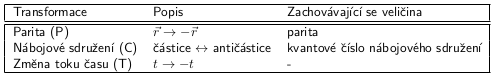
\includegraphics[width=0.8\textwidth]{Diskretnetran.png}
\caption{Diskretne transformacie a ich vlasatnosti.}
\label{sf1:fig:Diskretnetran}
\end{figure}
\newline
\textbf{CP symetria a jej narusenie}\par
Naznacili sme, ze slabe interakcie narusuju paritu (P) a aj nabojove zdruzenie (C). Povodne sa komunita fyzikov domnievala, ze kombinacia CP symetrie zostava slabymi interakciami nenarusena. Platilo by totiz $\hat{C}\hat{P}\nu_{L}=\hat{C}\nu_P=\nu_{\bar{P}}$.\par
V 50. rokoch vsak bolo narusenie CP symetrie navrhnuto ako reakcia na objavenie narusenia parity. 
K experimentálnemu potvrdeniu se dospelo v roku 1964 v BNL objavenim anomalii v rozpade neutralneho kaonu. Bolo totiz zistene, ze neutrlane kaony sa mozu premenit na svoje anti-castice a naopak, ale k tymto prechodom nedochadza s presne rovnakou pravdepodobnostou v oboch smeroch = mierne narusenie CP symetrie.\par
V roku 1968 prisiel A. Sacharov s myslienkou, ze by narusenie CP symetrie v silnej interakcii mohlo mat pri vzniku Vesmiru za nasledok prevladanie hmoty nad anti-hmotou. V obdobi pred Velkym zjednotenim interakcii castice X a Y prechody sposobovali nerovnosti medzi kvarkmy a leptonmy. Vdaka naruseniu CP invariancie v silnej interakcii prebiehali tieto procesy mierne nesymetricky a viedli  k velmi malemu poruseniu rovnovahy medzi hmotou a anti-hmotou. Zhruba na jednu miliardu reakcii oboma smermi prebehlo o jednu reakciu viac smerom k hmote. Ked sa Vesmir dostatocne ochladil. doslo k anihilacii latky s anti-latkou. Pri tejto anihilacii vsak na kazdu miliardu castic a anti-castic zostala kvoli naruseniu CP symetrie jedna castica hmoty. Prave z tychto castic je dnesny vesmir postaveny.\par
Narusenie CP symetrie bolo pozorovane az v roku 2004 na detektore BABAR na Stanforde. Pri zrazkach tu vznikali kvarky a anti-kvarky $b$. Sledovane boli rozpady castice $B^0$ a jej anticastice $\bar{B}^0$. Rozpad oboch castic ma možnost prebiehat vela moznostami, z nich bolo tiez mozne sledovat vzacny rozpad na dvojicu pion a kaon $B^0 \rightarrow K^+ \pi^-$ alebo $\bar{B}^0 \rightarrow K^- \pi^+$.\par
V pripade rovnakych vlastnosti hmoty a anti-hmoty by obe reakcie mali prebiehat rovnako pravdepodobne a mali by sa objavovat rovnake pocty kvarkov $K^- \pi^+$ a $K^+ \pi^-$. Skutocnost ale bola ina. V experimente bolo detekovano 910 parov $K^+ \pi^-$ a len  695 $K^- \pi^+$. Sposob rozpadu hmoty a anti-hmoty tak prebieha odlisne.\par
Narusenie CP symetrie je v Standartnom modely zahrnute zavedenim komplexnej fazy v CKM matici popisujucej miesanie kvarkov. V tomto schemate je pre komplexnu fazu, a tudiz narusenie CP symetrie, nevyhnutnou podmienkou existencia najmenej troch generacii kvarkov. Podla CPT teoremu odpoveda narusenie CP symetrie naruseniu invariancie vzhladom ku zmene toku casu. Keby CP bola skutocnou symetriou , potom by prirodne zakony platili rovnako ako pre hmotu tak aj pre anti-hmotu.
\newline 
\textbf{CPT teorem}\par
Vo fyziklanych javoch sa zachovava CPT symetria. Kombinacia vsetkych diskretnych transformacii sa poklada za nenarusenu vo vsetkych fundamentalnych interakciach a zaroven za zakladnu vlastnost fyzikalnych zakonov. CPT teoria konkretne prehlasuje, ze vsetky lokalne interagujuce polia, ktorych Lagrangiany su invariantne vo vlastnej Lorentzovskej transforamacii, su invariantne voci kombinovanej transformacii nabojoveho zdruzenia, parity a casovej inverzie. Experimentalne proverovanie tejto invariancie sa robilo porovnavanim vlastnosti castic s ich anti-casticami. Pokial je totiz CPT teorem spravny, kazda castica musi mat presne rovnaku hmotu a dobu zivota ako jej odpovedajuca anti-castica. Prebehlo mnoho merani parov castica-anticastica, najcitlivejsie overene rozdiely poskytol par $K^0-\bar{K}^0$, pozri obrazok \ref{sf1:fig:MeranieCPT}.
\begin{figure}[!h]
\centering
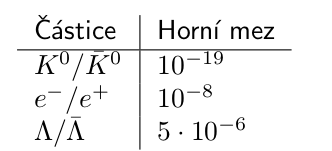
\includegraphics[width=0.3\textwidth]{MeranieCPT.png}
\caption{Relativne hmotnostne rozdiely medzi casticami a anti-casticami.}
\label{sf1:fig:MeranieCPT}
\end{figure} \newline
Relativne rozdiely medzi hmotnostami castic a anti-castic sa robilo pomocou $$\delta(m)=\frac{m-\bar{m}}{m+\bar{m}} $$.
Zo strednych dob zivota mionov bola stanovena horna medza pomerov na $$ \frac{\tau(\mu^+)-\tau(\mu^-)}{\tau(\mu^+)+\tau(\mu^-)}<10^{-4} $$. 
S velkou presnostou boli zmerane magneticke momenty elektronov-pozitron a mion-antimion. Vysledky su obvykle prezentovane v pojmoch gyromagnetickych faktorov $g$, ktorymi su vyjadrene magneticke momenty castic. Pre elektrony mame $$ \frac{g(e^+)-g(e^-)}{g(e+)+g(e^-)}<10^{-12} $$.
Obdobna velicina pre miony ma hornu medzu $10^{-8}$. Vsetky experimentalne dokazy podporuju invarianciu vsetkych interakcii voci transformacii CPT. Pokial je totiz invariancia niektorej z operacii narusena, musi byt kompenzovana ostatnymi transformaciami. Napriklad narusenie invariancie vzhladom k casovej inverzii, musi byt tiez narusena invariancia vzhladom k CP.\par
Dosledkom CPT symetrie je to, že se zrkadlový obraz našeho vesmíru, teda otočenie všetkych objektov s ich poziciami v lubovolnej rovině (odpovedajuce inverzi parity), obratenie všetkych hybností (odpovedajuce časovej inverzi) a nahradenie vsetkej hmoty antihmotou (co odpovedá nábojovej inverzi), bude vyvíjat presne podla známých fyzikálních zákonov. CPT transformacia zmení náš vesmír na jeho zrcadlový obraz a naopak. \par
Dosledkov platnosti CPT symetrie je hned niekolko
\begin{itemize}
	\item Castice s celociselnym spinom podliehaju Bose-Einsteinovej statistike, zatial co polociselne Fermi-Diracove statistike.
	\item Castice a ich anti-castice maju totozne hmotnosti a doby zivota.
	\item vsetky vnutorne cisla castic su opacne k vnutornym kvantovym cislam prisluchajucich anti-castic.
\end{itemize}

\section{Súradnicové sústavy v subjadrovej fyzike}
Transformace kinematických veličin mezi soustavami, Mandelstamovy proměnné,\newline
\textbf{Mandelstamovy premenne}\par
Mandelstamové premenné sú číselné veličiny, ktoré kódujú energiu, hybnosť a uhly častíc v rozptylovom procese Larentzovo-invariantným spôsobom. Používajú sa na rozptylové procesy dvoch častíc na dve častice, pozri obrazok \ref{sf1:fig:Mandelstam}. V Minkovskeho metrike diag(1,-1,-1,-1) maju tieto premenne nasledujuci tvar
\begin{equation}
\begin{gathered}
s=(p_1+p_2)^2=(p_3+p_4)^2 \\
t=(p_1-p_3)^2=(p_4-p_2)^2 \\
u=(p_1-p_4)^2=(p_3-p_2)^2
\end{gathered}
\end{equation}
\begin{figure}[!h]
\centering
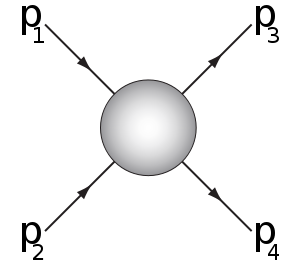
\includegraphics[width=0.2\textwidth]{Mandelstam.png}
\caption{V tomto diagrame castice s $p_1$ a $p_2$ prichadzaju a interaguju zatial co $p_3$ a $p_4$ odchadzaju z interakcie.}
\label{sf1:fig:Mandelstam}
\end{figure}
Kazdej z tychto premennych odpoveda urcita topologia zrazky. Tieto typy odpovedaju roznym Feynmanovym diagramom. s-kanal, t-kanal, u-kanal, pozri obrazok \ref{sf1:fig:Kanaly}.
\begin{figure}[!h]
\centering
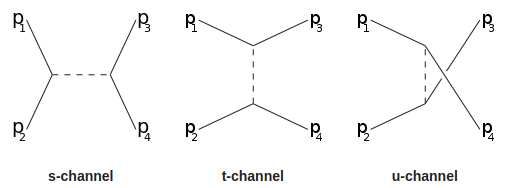
\includegraphics[width=0.6\textwidth]{Kanaly.png}
\caption{s, t, u -kanaly. s-kanál je jediný spôsob, akým môžu byť objavené rezonancie a nové nestabilné častice za predpokladu, že ich životnosť je dostatočne dlhá a že sú priamo zistiteľné. t-kanál predstavuje proces, v ktorom častica 1 emituje intermedialnu časticu a stáva sa konečnou časticou 3, zatiaľ čo častica 2 absorbuje intermedialnu časticu a stáva sa 4. Pre u-kanal zamenime v t-kanaly len 3 a 4. 
}
\label{sf1:fig:Kanaly}
\end{figure}
\newline
V relativistickej limite zanedbame hmotnosti oproti hybnosti $p^2 >>> (m_0c^2)^2$.\par
Suma Mandelstam-ovych premennych nam da sumu hmotnosti castic. $$ s+t+u=m_1^2+m_2^2+m_3^2+m_4^2 $$\newline
\textbf{Lorentzovske transformacie}\par
Uvazujme dve kartezske vztazne sustavy $S$ a $S^{\prime}$, tak ze ich pociatky splivaju v case $t=t^{\prime}=0$. Suradnicove osy oboch sustav su vzajomne rovnobezne a pohybuju sa tak, ze sustava $S$ (kludova) zostava v pokoji a sustava $S^{\prime}$ sa vzhladom na $S$ hybe rychlostou $v$ v kladnom smere osy $x$. Lorentzove transformacie potom su 
\begin{equation} 
x^{\prime}=\frac{x-vt}{\sqrt{1-\frac{v^2}{c^2}}},\hspace{0.3cm} y^{\prime}=y,\hspace{0.3cm} z^{\prime}=z,\hspace{0.3cm} t^{\prime}=\frac{t-\frac{vx}{c^2}}{\sqrt{1-\frac{v^2}{c^2}}} 
\end{equation}
kde $\beta=v/c$ a $c$ je ryclost svetla vo vakuum. Pre transformacie energie a hybnosti z jednej do druhej sustavy dostavame 
\begin{equation}
E^{\prime]}=\frac{E-p_xv}{\sqrt{1-\frac{v^2}{c^2}}}, \hspace{0.8cm} p_x^{\prime}=\frac{p_x-\frac{vE}{c^2}}{\sqrt{1-\frac{v^2}{c^2}}}
\end{equation}\newline
\textbf{Kinematika zrazkovych procesov}\par
Experimentalne zrazkove procesy: experiment s pevnym tercom, experiment s naproti iducimi zvazkamy, pozri obrazok \ref{sf1:fig:Zrazky}.
\begin{figure}[!h]
\centering
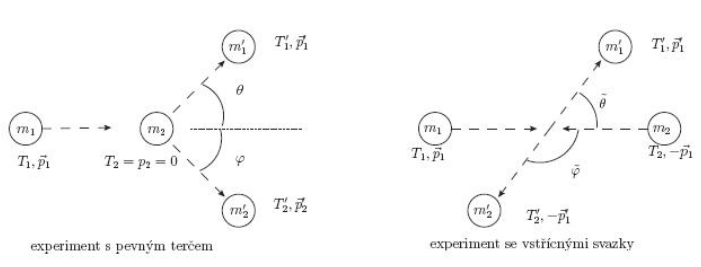
\includegraphics[width=0.8\textwidth]{Zrazky.png}
\caption{Rozne druhy zrazkovych procesov. Vlavo Lab frame a vpravo CMS frame.}
\label{sf1:fig:Zrazky}
\end{figure}
Sustavy su pred aj po interakcii izolovane. Oblast, kde sa castice stretnu a interaguju sa nazyva $interakcna$ $oblast$. Mimo tuto oblast sa castice pohybuju volne (realne je sila interakcie zanedbatelne mensia ako pre oblast interakcie). Budeme pouzivat znacenie velicin nasledovne: pred interakciou budu veliciny bez ciarky a po zrazke s ciarkou.\par
Zakony zachovania energie a celkovej hybnosti izolovanej sustavy mozme napisat v tvare: $E=E^{\prime}$ a $\vec{P}=\vec{P}^{\prime}$. Podla produktov rozlisujeme nasledujuce dva druhy interakcii
\begin{itemize}
	\item \textbf{pruzny rozptyl}: nemenia sa kludove hmotnosti ani typy castic po interakcii. Zo zakona zachovania energie plynie, ze celkova kineticka energia sa zachovava.
	\item \textbf{nepruzny rozptyl}: pri interakcii sa menia hmotnosti zucastnenych castic. Velicinu $Q=[(m_1+m_2)^2-(m_1^{\prime}+m_2^{\prime})^2]=(M-M^{\prime})^2$ nazyvame energia interakcie. Zo zakona zachovania plynie $T^{\prime}=T+Q$. Pre nepruznu interakciu je $Q$ nerovne nule a naopak pre pruznu zrazku je to $Q$ nulove. 
\end{itemize}
\textbf{Suradnicove systemy}\par
\begin{itemize}
	\item \textbf{Laboratorna sustava} - tato sustava je pevne spojena s detektorom. Jej pouzitie nie je vzdy vhodne, kedze vztahy popisujuce interakciu su v nej dost zlozite. V tejto sustave sa meraju hlavne experimenty s pevnym tercom. Avsak nemusi to byt vzdy sustava spojena s detektorom. Pouziva sa aj laboratorna sustava spojena s nejakou casticou, s ktorou ma druha castica interagovat.
	\item \textbf{Taziskova sustava (CMS)} - tato sustava je v pokoji. Zaujima nas len relativny pohyb castic. Celkova hybnost castic je rovna nule, co dost moze zjednodusit vypocet.
	\item \textbf{Tercikova sustava} - sustava v ktorej je hybnost terca nulova.
	\item \textbf{Sustava zvazku} - sustava, v ktorej je hybnost zvazku nulova.
	\item \textbf{Coliding beam frame} - sustava, v ktorej sa zvazky zrazaju pod uhlom $\theta$.
\end{itemize}
Kineticku energiu v laboratornej sustave je mozne rozdelit na cast, ktora prislucha translacnemu pohybu sustavy castic - (kineticku energiu taziska) a cast, ktora prislucha relativnemu pohybu castic-(kineticka energia v taziskovej sustave). Kinematicke vztahy v taziskovej sustave sa vyznacuju maximalnou symetriou, co je jednoduchsie na vypocty. Vzhladom k tomu, ze vacsina experimentalnych vysledkov je ziskana v laboratornej sustave, je nutne medzi taziskovou a laboratornou sustavou prechadzat.\par
Zapiseme zakon zachovania hybnosti, zakon zachovania energie a rychlosti taziska v laboratornej sustave
\begin{equation}
\begin{gathered}
\vec{p_1}+\vec{p_2}=\vec{p_1}^{\prime}+\vec{p_2}^{\prime} \\
T_1+T_2=T_1^{\prime}+T_2^{\prime} \\
\vec{v}_T=\frac{m_1\vec{v}_1+m_2\vec{v}_2}{m_1+m_2}.
\end{gathered}
\end{equation}
Teraz uvedieme zakony zachovania a ryclost taziska v taziskovej sustave
\begin{equation}
\begin{gathered}
\tilde{\vec{p}}_1+\tilde{\vec{p}}_2=\tilde{\vec{p}}_1^{\prime}+\tilde{\vec{p}}_2^{\prime}=0 \\
\tilde{T}_1+\tilde{T}_2=\tilde{T}_1^{\prime}+\tilde{T}_2^{\prime} \\
\vec{v}_T=0.
\end{gathered}
\end{equation}
z coho plynie $$ \lvert \tilde{\vec{p}}_1 \rvert=\lvert \tilde{\vec{p}}_2 \rvert=\lvert \tilde{\vec{p}}_1 \rvert=\lvert \tilde{\vec{p}}_2  \rvert, \hspace{0.3cm} \tilde{\vec{v}}_1=\tilde{\vec{v}}_1^{\prime}, \hspace{0.3cm} \tilde{\vec{v}}_2=\tilde{\vec{v}}_2^{\prime}, \hspace{0.3cm} \tilde{T}_1=\tilde{T}_1^{\prime}, \hspace{0.3 cm} \tilde{T}_2=\tilde{T}_2^{\prime}. $$
Za predpokladu, ze je v laboratornej sustave tercikova castica v klidu ($p_2=0, T_2=0$), potom plati
\begin{equation}
\begin{gathered}
\tilde{\vec{v}}_1=\vec{v}_1-\vec{v}_T=\vec{v}_1-\frac{m_1\vec{v}_1+m_2\vec{v}_2}{m_1+m_2}=\frac{m_2}{m_1+m_2}\vec{v}_1\rightarrow \tilde{\vec{p}}_1=\mu \vec{v}_1 \\
\tilde{\vec{v}}_2=\vec{v}_2-\vec{v}_T=\vec{v}_2-\frac{m_1\vec{v}_1+m_2\vec{v}_2}{m_1+m_2}=-\frac{m_1}{m_1+m_2}\vec{v}_1\rightarrow \tilde{\vec{p}}_2=-\mu \vec{v}_1 \\
\tilde{T}=\tilde{T}_1+\tilde{T}_2=\frac{\tilde{p}_1^2}{2m_1}+\frac{\tilde{p}_2^2}{2m_2}=\frac{1}{2}\mu v_1^2=\frac{m_2}{m_1+m_2}T_1
\end{gathered}
\end{equation}
kde $\mu=\frac{m_1m_2}{m_1+m_2}$ je redukovana hmotnost. Toto su vztahy prechodu medzi taziskovou a laboratornou sustavou.

\section{Kinematické premenné}
Uvazujeme ze $c=\hbar=1$.\newline
Majme proces $a+b\rightarrow c+X$, kde $X$ su nespecifikovane castice. Casticu $c$ mozme povazovat za dcersku casticu od castice $a$ alebo $b$. Zrazku castic budeme uvazovat v sustave, kde zvazok casic $a$ nalietava v smere osi $z$ na terc tvoreny casticami $b$.\newline
Oznacme 
\begin{equation}
\begin{gathered}
p_a=(E_a,\vec{p}_{Ta},p_{za})\hspace{0.6cm} 4-impulz\hspace{0.2cm} nalietavajucej \hspace{0.2cm} castice \\
p_b=(E_b,\vec{p}_{Tb},p_{zb})\hspace{0.6cm} 4-impulz\hspace{0.2cm} tercikovej \hspace{0.2cm} castice,
\end{gathered}
\end{equation}
kde sme zaviedli tkz. priecnu hybnost, ktora je definovana ako $p_T=p\sin(\theta)$, kde $\theta$ je uhol rozptylu.\par
Hladame premenne, ktore su zlozene zo zloziek 4-impulzu castice (ktoru meriame) a maju nejaku specialnu vlastnost pri Lorentzovskej transformacii (co nam velmi zjednodusi popis). Pre detekovanu dcersku casticu $c$ definujeme
\begin{equation}
\begin{gathered}
c_+=E_c+p_{zc} \hspace{0.6cm} forward \hspace{0.2cm} lightcone \hspace{0.2cm} momentum \\
c_-=E_c-p_{zc} \hspace{0.6cm} backward \hspace{0.2cm} lightcone \hspace{0.2cm} momentum.
\end{gathered}
\end{equation}
Pre pomer dvoch lightcone premennych plati (zaroven to je Lorentzovky invariant)
$$ x_{\pm}=\frac{E_c\pm p_{cz}}{E_b\pm p_{bz}} \hspace{0.3cm} 0<x_{\pm}<1, $$ 
kde $x_{\pm}$ je forward (backward) lightcone premenna castice $c$ vzhladom k castici $b$.\par
Rovnako by sme mohli zavies $x_{\pm}$ vzhladom na casticu $a$ pretoze nie vzdy je mozne povedat, ktora castica je materskou casticou. Pokial skumame experiment, ktory produkuje castice v jednom preferovanom smere, berieme obvykle len jednu z lightcone premennych, druha sa nepouziva.\newline

\textbf{Rapidita}\par
Rapidita je bezrozměrná fyzikální veličina, která je mírou pohybu prostorem, podobně jako rychlost. Zatímco rychlost objektů je podle speciální teorie relativity shora omezena rychlostí světla ve vakuu $c$, rapidita může být libovolně velká. Pro objekty v klidu má hodnotu 0 a pro pomalé objekty je přímo úměrná rychlosti. Když se rychlost objektu přibližuje $c$, roste rapidita nade všechny meze.
Je definovana nasledovne $$ y=\frac{1}{2}\ln\bigg( \frac{E+p_z}{E-p_z} \bigg)=\frac{1}{2}\ln\bigg( \frac{x_+}{x_-} \bigg), $$
v nerelativisticke limite $y\rightarrow \beta$. Rapidita nie je lorentzovsky invariant, ale transformuje sa ako $\tilde{y}=y-y_{\beta}$ kde $y_{\beta}$ je rychlost pohybujucej sa vztaznej sustavy $S^{\prime}$.\par
Dalej plati
\begin{equation}
\begin{gathered}
E=m_T\cosh(y) \\
p_z=m_T\sinh(y),
\end{gathered}
\end{equation}
kde velicina $m_T$ je tzv. priecna hmotnost a je definovana nasledujucim sposobom
$$ m^2=E^2-p^2=E^2-p_z^2-p_T^2 \hspace{0.2cm} \rightarrow \hspace{0.2cm} E^2-p^2_z=m^2+p^2_T=m^2_T. $$\newline
\newpage
\textbf{Pseudorapidita}\par
Jej vyhodou je oproti rapidite v tom, ze staci jedna premenna pre jej definiciu - uhol vyletu. Pseudorapidita je definovana nasledovne
$$ \eta=-\ln\bigg( \tan\frac{\theta}{2}  \bigg) = \frac{1}{2}\ln \bigg( \frac{\lvert \vec{p} \rvert+p_z}{\lvert \vec{p} \rvert-p_z} \bigg), $$
kde uhol $\theta$ je uhol medzi hybnostou castice $\vec{p}$ a osou zvazku. V druhej casti vztahu mozme vidiet, ze pre velke hybnosti (resp. male hmotnosti) rapidita a pseudorapidita splyvaju ($p\approx E$).
\begin{figure}[!h]
\centering
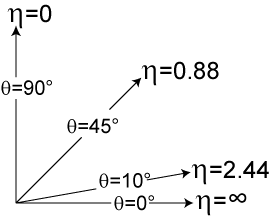
\includegraphics[width=0.3\textwidth]{Pseudorapidity.png}
\caption{Tu mozme vidiet ako sa pseudorapidita meni s uhlom $\theta$.}
\label{sf1:fig:Pseudorapidity}
\end{figure}
\newline

\textbf{Feynmanova promenna}\par
Bola zavedena pri sudiu vysoko-energetickych zrazok hadronov pre popis elementarnej interakcie na kvarkovej urovni. Je definovana vztahom $$ x_F=\frac{\tilde{p}_z}{\tilde{p}_z^{max}}. $$
Feynmanova premenna je obvykle definovana v sustave, v ktorej sa castica pohybuje s nekonencou hybnostou (infinite momentum frame). Je tomu tak preto, lebo v kvantovej mechanike nie je operator poctu castic invariantny voci prechodu z jednej sustavy do druhej, a tak pocet castic, ktore pozorujeme pri lete vysoko-energetickej castice, zavisi na sustave, v ktorej proces studujeme. Limitna sustava je potom sustava, kde sa vsetky castice pohybuju s nekonecnou hybnostou, a tak doba zivota kvantovo vytvorenych castic je nekonecne mala a je tak mozne dobre definovat casticove obsadenie sustavy.\par
V tejto sustave mozeme ukazat,, ze $x_F=\frac{2\tilde{p}_z}{\sqrt{s}},$ dalej tiez plati $0<x_F<1$ a pre $E\rightarrow \infty$ mame $x_F=1$.\newline

\textbf{Bjorkenova promenna}\par
Jeto velicina, ktoa je definovana nasledovne $$ x=\frac{Q^2}{2(p_2\cdot q)}, $$ kde $Q^2=-q^2$. Na obrazku \ref{sf1:fig:Bjorken} su znazornene jednotlive 4-impulzy vyskytujuce sa v tejto premenne.
\begin{figure}[!h]
\centering
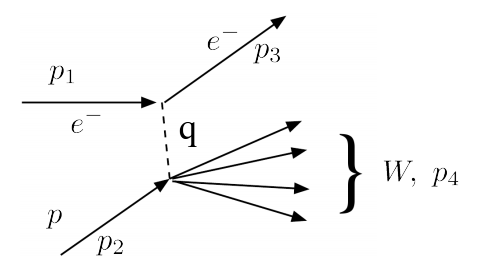
\includegraphics[width=0.6\textwidth]{Bjorken.png}
\caption{Rozptyl elektronu na protone.}
\label{sf1:fig:Bjorken}
\end{figure}
Podla obrazka mame
$$ p_4^2=M_W^2=(q+p_2)^2=q^2+2qp_2+p_2^2=-Q^2+2qp_2+M_p^2\rightarrow Q^2=2qp_2+M_p^2-M_W^2, $$
kedze je $M_p$ hmotnost protonu, ktory je najlahsi baryon, a $M_W$ hmotnost akehokolvek ineho baryonu tak $Q^2$ nebude nikd viac ako $2qp_2$.
Potom mame pre neelasticky rozptyl: $0<x<1$, zatial co pre elasticky rozptyl $x=1$.\par
($1-x$) ako keby reprezentovala cast prenesenej enegie, ktora sa spotrbuje na vytvorenie tazsieho baryonu (avsak toto je len moj nazor takze treba na to pozerat z nadhladom).

\end{document}